\documentclass[11pt]{article}

% ------------------------------------------------------------------
% Packages
% ------------------------------------------------------------------
\usepackage[letterpaper,margin=1in]{geometry}
\usepackage[T1]{fontenc}
\usepackage{lmodern}
\usepackage{microtype}
\usepackage{amsmath,amssymb,amsthm,mathtools,bm}
\usepackage{graphicx}
\usepackage{booktabs,array,tabularx}
\usepackage{enumitem}
\usepackage[dvipsnames]{xcolor}
\usepackage[most]{tcolorbox}
\usepackage{caption}
\usepackage[titles]{tocloft}
\setlength{\cftbeforesecskip}{0.5em}
\usepackage[colorlinks=true,linkcolor=RoyalBlue,citecolor=OliveGreen,urlcolor=RoyalBlue]{hyperref}
\usepackage[capitalise,nameinlink,noabbrev]{cleveref}

\captionsetup{font=small,labelfont=bf}
\setlist{itemsep=2pt,topsep=4pt}
\numberwithin{equation}{section}
\setlength{\parskip}{3pt}

% ------------------------------------------------------------------
% Theorem-like environments (one shared counter per section)
% ------------------------------------------------------------------
\theoremstyle{plain}
\newtheorem{theorem}{Theorem}[section]
\newtheorem{lemma}[theorem]{Lemma}
\newtheorem{proposition}[theorem]{Proposition}
\newtheorem{corollary}[theorem]{Corollary}
\theoremstyle{definition}
\newtheorem{definition}[theorem]{Definition}
\newtheorem{example}[theorem]{Example}
\newtheorem{assumption}{Assumption}
\renewcommand{\theassumption}{A\arabic{assumption}}
\theoremstyle{remark}
\newtheorem{remark}[theorem]{Remark}
\crefname{assumption}{Assumption}{Assumptions}

% Boxes for the key statements
\tcbset{keybox/.style={enhanced,breakable,colback=RoyalBlue!4,colframe=RoyalBlue!60!black,
  boxrule=0.6pt,arc=2pt,left=6pt,right=6pt,top=4pt,bottom=4pt}}
\tcbset{intuition/.style={enhanced,breakable,colback=Goldenrod!8,colframe=Goldenrod!70!black,
  boxrule=0.5pt,arc=2pt,left=6pt,right=6pt,top=3pt,bottom=3pt,fonttitle=\bfseries\small,
  coltitle=black,colbacktitle=Goldenrod!25}}

% ------------------------------------------------------------------
% Notation
% ------------------------------------------------------------------
\newcommand{\R}{\mathbb{R}}
\newcommand{\E}{\mathbb{E}}
\newcommand{\Ek}{\mathbb{E}_k}
\newcommand{\norm}[1]{\lVert #1\rVert}
\newcommand{\Norm}[1]{\bigl\lVert #1\bigr\rVert}
\newcommand{\ip}[2]{\langle #1,\, #2\rangle}
\newcommand{\fs}{f^\star}
\newcommand{\eps}{\varepsilon}
\newcommand{\Dlt}{\Delta}
\newcommand{\cb}{c_\beta}
\newcommand{\ie}{i.e.,\ }
\newcommand{\eg}{e.g.,\ }

\hypersetup{pdftitle={Convergence of Stochastic Gradient Descent with Momentum},
  pdfsubject={Expected-decrease analysis of SGD with momentum (stochastic heavy ball)},
  pdfkeywords={SGD, momentum, heavy ball, Lyapunov function, nonconvex optimization, convergence}}

\title{\textbf{Convergence of Stochastic Gradient Descent with Momentum}\\[4pt]
  \large An expected-decrease analysis in the style of SGD, with complete proofs,\\
  and a map of when convergence holds}
\author{SGDM\_Proof project}
\date{October 2026}

\begin{document}
\maketitle

\begin{abstract}
\noindent
Stochastic gradient descent with momentum (SGDM, also called the stochastic heavy-ball
method) is a default optimizer in machine learning, yet its convergence proof is far less
familiar than the textbook proof for plain SGD. The obstacle is that momentum lets the
iterates overshoot, so the function value $f(x_k)$ need not decrease---not even in
expectation, and not even without noise. This report shows how to recover an SGD-style
\emph{expected decrease inequality} for SGDM by measuring progress with a
potential that combines the function value at an extrapolated point with a kinetic-energy
term. From this single inequality we derive, with every step written out:
(i)~convergence to stationary points of smooth nonconvex functions at the same
$O(1/\sqrt{K})$ rate as SGD; (ii)~convergence with diminishing step sizes; (iii)~linear
convergence up to a noise floor, and an $O(1/k)$ rate with decaying steps, under the
Polyak--{\L}ojasiewicz condition; and (iv)~an $O(1/\sqrt{K})$ rate for convex functions
under a milder step-size condition. We then map out \emph{when} these guarantees hold: we
compute the noise floor exactly on quadratics, derive the exact stability region of the
heavy-ball method on quadratics, prove that without noise a mechanical energy decreases for
every smooth function when $\alpha<2(1-\beta)/L$, and verify by hand a classical
counterexample in which momentum parameters tuned for quadratics make the method cycle on a
strongly convex function. Numerical experiments illustrate each statement. Only
multivariable calculus, linear algebra and basic probability are assumed.
\end{abstract}

\newpage
{\small\setlength{\parskip}{0pt}\tableofcontents}
\newpage

% ======================================================================
\section{Introduction}\label{sec:intro}
% ======================================================================

\subsection{The problem and the two algorithms}

We want to solve the unconstrained minimization problem
\begin{equation}\label{eq:problem}
  \min_{x\in\R^d} f(x),
\end{equation}
where $f:\R^d\to\R$ is differentiable, but its gradient $\nabla f$ is not available
exactly. Instead, at any point $x$ we can ask for a \emph{stochastic gradient}
$g(x;\xi)$: a random vector, depending on a random sample $\xi$, which is correct
\emph{on average}, $\E_\xi[g(x;\xi)]=\nabla f(x)$. This is the situation in machine
learning, where $f(x)=\frac1n\sum_{i=1}^n f_i(x)$ is the average loss over $n$ training
examples and $g(x;\xi)=\nabla f_\xi(x)$ is the gradient of the loss on one randomly chosen
example (or on a random mini-batch).

\paragraph{SGD.} Stochastic gradient descent starts at a point $x_0$ and repeats
\begin{equation}\label{eq:sgd}
  x_{k+1}=x_k-\alpha\, g_k,\qquad g_k:=g(x_k;\xi_k),\qquad k=0,1,2,\dots
\end{equation}
where $\alpha>0$ is the \emph{step size} (learning rate) and $\xi_0,\xi_1,\dots$ are
independent samples.

\paragraph{SGDM.} SGD with momentum---also called the \emph{stochastic heavy-ball
method}, after Polyak's heavy-ball method~\cite{polyak1964}---adds a fraction
$\beta\in[0,1)$ of the previous displacement:
\begin{equation}\label{eq:sgdm-intro}
  x_{k+1}=x_k-\alpha\, g_k+\beta\,(x_k-x_{k-1}),\qquad x_{-1}:=x_0 .
\end{equation}
Physically, $x_k$ is the position of a heavy ball rolling down the graph of $f$: the term
$\beta(x_k-x_{k-1})$ is its inertia (it keeps moving in the direction it was already
moving), and $1-\beta$ plays the role of friction. With $\beta=0$ we recover SGD. In deep
learning, \eqref{eq:sgdm-intro}---usually implemented in an equivalent ``momentum buffer''
form (\cref{sec:forms})---with $\beta=0.9$ is a standard default~\cite{sutskever2013}.

\subsection{What ``convergence'' means here}

For a nonconvex $f$ there is no efficient method that is guaranteed to find a global
minimizer, so the standard goal is an approximate \emph{stationary point}, a point with a
small gradient. Since the iterates are random, guarantees are stated in expectation. A
typical statement has the form
\[
  \min_{0\le k<K}\E\norm{\nabla f(x_k)}^2\;\le\;(\text{a quantity that tends to $0$ as
  $K\to\infty$}),
\]
and the speed at which the right-hand side decreases in the number of iterations $K$ is
the \emph{rate}. For special classes of functions (Polyak--{\L}ojasiewicz or convex) we
will also bound the optimality gap $\E[f(x_k)]-\fs$, where $\fs=\inf f$.

\subsection{The difficulty, and the idea in one line}

For SGD, every textbook proof~\cite{bottou2018,ghadimilan2013} rests on one inequality,
the \emph{expected decrease}:
\begin{equation}\label{eq:intro-sgd-decrease}
  \E\bigl[f(x_{k+1})\,\big|\,\text{history}\bigr]\;\le\;f(x_k)
  -\frac{\alpha}{2}\norm{\nabla f(x_k)}^2+\frac{L\alpha^2}{2}\sigma^2
  \qquad(\alpha\le 1/L),
\end{equation}
where $L$ is the smoothness constant of $f$ and $\sigma^2$ bounds the variance of the
stochastic gradients (\cref{sec:sgd}). In words: on average, one step decreases $f$ by an
amount proportional to the squared gradient, minus a price for the noise that is
\emph{quadratic} in the step size. Everything else---rates, step-size rules---follows by
summing \eqref{eq:intro-sgd-decrease} over $k$.

For SGDM, inequality \eqref{eq:intro-sgd-decrease} is \emph{false}, even without noise:
momentum can carry the iterate uphill (in \cref{ex:overshoot} the method sits exactly at
the minimizer and is pushed away by its own inertia). It holds only at steps where the
momentum still points downhill (\cref{prop:f-step}), and the algorithm cannot control
when that is the case. The function value is the wrong yardstick. The idea of this report is to measure progress with a \emph{potential}
\[
  \Phi_k=f(z_k)-\fs+\frac{L\beta^2}{2(1-\beta)^2}\norm{x_k-x_{k-1}}^2,
  \qquad z_k=x_k+\frac{\beta}{1-\beta}\,(x_k-x_{k-1}),
\]
where $z_k$ is an extrapolated point---the place where the ball would come to rest if all
forces were switched off (\cref{sec:extrapolated})---and the second term is a kinetic
energy. We prove (\cref{thm:master}) that $\Phi_k$ obeys the exact analogue of
\eqref{eq:intro-sgd-decrease}:
\begin{tcolorbox}[keybox]
\begin{equation}\label{eq:intro-master}
  \E\bigl[\Phi_{k+1}\,\big|\,\text{history}\bigr]\;\le\;\Phi_k
  -\frac{\gamma}{4}\norm{\nabla f(x_k)}^2+L\gamma^2\sigma^2,
  \qquad \gamma:=\frac{\alpha}{1-\beta},
\end{equation}
\centering whenever the step size satisfies $\displaystyle\alpha\le\frac{(1-\beta)^2}{2L}$.
\end{tcolorbox}
\noindent Once \eqref{eq:intro-master} is available, all the standard SGD conclusions
transfer to SGDM by the same telescoping arguments, with the \emph{effective step size}
$\gamma=\alpha/(1-\beta)$ playing the role of $\alpha$.

\subsection{Summary of results}

\Cref{tab:summary} lists what we prove. Throughout, $\Dlt:=f(x_0)-\fs$, $\gamma=\alpha/(1-\beta)$,
and ``nonconvex'' means only that $f$ is $L$-smooth and bounded below.

\begin{table}[ht]
\centering\small
\renewcommand{\arraystretch}{1.25}
\begin{tabularx}{\textwidth}{@{}l l >{\raggedright\arraybackslash}X l@{}}
\toprule
Setting & Step-size condition & Guarantee & Where\\
\midrule
Nonconvex & $\alpha\le\frac{(1-\beta)^2}{2L}$ &
  $\frac1K\sum_{k<K}\E\norm{\nabla f(x_k)}^2\le\frac{4\Dlt}{\gamma K}+4L\gamma\sigma^2$ &
  \cref{thm:nonconvex}\\
Nonconvex, tuned $\gamma$ & $\gamma=\min\bigl\{\frac{1-\beta}{2L},\frac1\sigma\sqrt{\frac{\Dlt}{LK}}\bigr\}$ &
  $\frac1K\sum_{k<K}\E\norm{\nabla f(x_k)}^2\le\frac{8L\Dlt}{(1-\beta)K}+8\sigma\sqrt{\frac{L\Dlt}{K}}$ &
  \cref{cor:rate}\\
Nonconvex, decaying & $\gamma_k\le\frac{1-\beta}{2L}$, $\sum\gamma_k=\infty$, $\sum\gamma_k^2<\infty$ &
  $\liminf_k\norm{\nabla f(x_k)}=0$ almost surely &
  \cref{thm:diminishing}\\
No noise ($\sigma=0$) & $\alpha=\frac{(1-\beta)^2}{2L}$ &
  $\Phi_k$ non-increasing; $\min_{k<K}\norm{\nabla f(x_k)}^2\le\frac{8L\Dlt}{(1-\beta)K}$ &
  \cref{cor:deterministic}\\
No noise, smooth & $\alpha<\frac{2(1-\beta)}{L}$ &
  energy decreases; $\nabla f(x_k)\to0$ &
  \cref{prop:energy}\\
PL inequality & $\alpha\le\frac{(1-\beta)^2}{2L}$ &
  $\E f(x_k)-\fs\le2\bigl(1-\frac{\gamma\mu}{4}\bigr)^k\Dlt+\frac{8L\gamma\sigma^2}{\mu}$ &
  \cref{thm:pl}\\
PL, decaying & $\gamma_k=\frac{8}{\mu(k+a)}$ &
  $\E f(x_k)-\fs=O(1/k)$ &
  \cref{cor:pl-decay}\\
Convex & $\alpha\le\frac{1-\beta}{2L}$ &
  $\E f(\bar x_K)-\fs\le\frac{\norm{x_0-x^\star}^2}{\gamma K}+\frac{2\beta\Dlt}{(1-\beta)K}+\gamma\sigma^2$ &
  \cref{thm:convex}\\
\bottomrule
\end{tabularx}
\caption{Summary of the guarantees proved in this report (all for SGDM in heavy-ball form
with momentum $\beta\in[0,1)$; for $\beta=0$ they reduce to the corresponding SGD results
up to constants). The question ``under what circumstances?'' is discussed in
\cref{sec:circumstances}: there we show that the noise floor $\propto\gamma\sigma^2$ is
unavoidable with a constant step (\cref{prop:noise-floor}), that too large a step size
makes the method diverge or cycle (\cref{prop:quadratic-stability},
\cref{ex:lrp}), and how the admissible step sizes shrink as $\beta\to1$
(\cref{fig:regions}).}
\label{tab:summary}
\end{table}

\subsection{How to read this report}

\paragraph{Prerequisites.} Multivariable calculus (gradients, the chain rule, the
fundamental theorem of calculus), linear algebra (inner products, norms, eigenvalues of
$2\times2$ matrices) and probability (expectation, independence, and conditional
expectation at the level of ``average over what is not yet known''). \Cref{sec:prelim}
collects every tool we use, with proofs; later proofs cite these facts explicitly.

\paragraph{Road map.} \Cref{sec:sgd} reviews the SGD analysis, which serves as the
template. \Cref{sec:momentum} introduces SGDM, explains why the function value is the
wrong yardstick, and introduces the extrapolated point $z_k$. \Cref{sec:master}, the heart
of the report, proves the expected decrease inequality \eqref{eq:intro-master}.
\Cref{sec:convergence} turns it into convergence theorems. \Cref{sec:circumstances}
answers the question ``under what circumstances does SGDM converge?'', including exact
computations that show which parts of the conditions cannot be removed.
\Cref{sec:experiments} illustrates everything numerically; the code that produces every
figure is in the \texttt{experiments/} folder of the repository.

\paragraph{Relation to the literature.} The extrapolated-point (``virtual sequence'')
technique and potentials of this type are classical in analyses of momentum
methods~\cite{ghadimi2015,yang2016,yu2019,liu2020,sebbouh2021}. The aim here is a
self-contained, fully explicit version---one potential, one key inequality, and explicit
constants---written so that each line can be checked by hand. Constants are chosen for
readability, not optimized.

% ======================================================================
\section{Preliminaries}\label{sec:prelim}
% ======================================================================

This section collects every tool used later. Each fact comes with a short proof, so that
the main arguments can be checked line by line.

\subsection{Notation}

Vectors live in $\R^d$. For $a,b\in\R^d$, $\ip{a}{b}=\sum_{i=1}^d a_ib_i$ is the inner
product and $\norm{a}=\sqrt{\ip{a}{a}}$ the Euclidean norm. For $f:\R^d\to\R$ we write
$\fs:=\inf_{x\in\R^d}f(x)$ (possibly not attained). Sums $\sum_{k<K}$ run over
$k=0,1,\dots,K-1$. For SGDM we will use the following names, all defined precisely in
\cref{sec:momentum}:
\begin{center}\small
\begin{tabular}{@{}ll@{}}
\toprule
$\alpha>0$, $\beta\in[0,1)$ & step size and momentum parameter\\
$\gamma=\alpha/(1-\beta)$ & effective step size\\
$v_k=x_k-x_{k-1}$ & velocity (last displacement), $v_0=0$\\
$z_k=x_k+\frac{\beta}{1-\beta}v_k$ & extrapolated point\\
$\cb=\frac{L\beta^2}{2(1-\beta)^2}$ & weight of the kinetic energy\\
$\Phi_k=f(z_k)-\fs+\cb\norm{v_k}^2$ & potential\\
$\eps_k=g_k-\nabla f(x_k)$ & gradient noise\\
$\Dlt=f(x_0)-\fs$ & initial optimality gap\\
\bottomrule
\end{tabular}
\end{center}

\subsection{Elementary inequalities}

\begin{lemma}[Elementary facts]\label{lem:elementary}
For all $a,b\in\R^d$:
\begin{enumerate}[label=\textup{(\alph*)}]
  \item \emph{(Cauchy--Schwarz)} $|\ip{a}{b}|\le\norm{a}\norm{b}$.
  \item \emph{(Young)} For every $\rho>0$:
        $\ip{a}{b}\le\frac{\rho}{2}\norm{a}^2+\frac{1}{2\rho}\norm{b}^2$.
  \item \emph{(Polarization)} $-\ip{a}{b}=\frac12\norm{a-b}^2-\frac12\norm{a}^2-\frac12\norm{b}^2$.
  \item \emph{(Convexity of $\norm{\cdot}^2$)} For every $\theta\in[0,1]$:
        $\norm{\theta a+(1-\theta)b}^2\le\theta\norm{a}^2+(1-\theta)\norm{b}^2$.
  \item $\norm{a+b}^2\le2\norm{a}^2+2\norm{b}^2$.
  \item \emph{(Geometric series)} For $q\in[0,1)$ and $k\ge1$:
        $\sum_{j=0}^{k-1}q^j=\frac{1-q^k}{1-q}\le\frac{1}{1-q}$.
\end{enumerate}
\end{lemma}

\begin{proof}
(a) is the Cauchy--Schwarz inequality from linear algebra.
(b) $0\le\Norm{\sqrt\rho\,a-b/\sqrt\rho}^2=\rho\norm{a}^2-2\ip{a}{b}+\norm{b}^2/\rho$;
rearrange and divide by $2$.
(c) Expand $\norm{a-b}^2=\norm{a}^2-2\ip{a}{b}+\norm{b}^2$ and rearrange.
(d) Expanding both sides,
\[
\theta\norm{a}^2+(1-\theta)\norm{b}^2-\norm{\theta a+(1-\theta)b}^2
=\theta(1-\theta)\bigl(\norm{a}^2-2\ip{a}{b}+\norm{b}^2\bigr)=\theta(1-\theta)\norm{a-b}^2\ge0 .
\]
(e) Apply (d) with $\theta=\frac12$ to the vectors $2a$ and $2b$:
$\norm{a+b}^2=\norm{\tfrac12(2a)+\tfrac12(2b)}^2\le\tfrac12\norm{2a}^2+\tfrac12\norm{2b}^2$.
(f) Multiply $\sum_{j=0}^{k-1}q^j$ by $1-q$; the sum telescopes to $1-q^k\le1$.
\end{proof}

\subsection{Smooth functions and the descent lemma}

\begin{definition}[$L$-smoothness]\label{def:smooth}
A differentiable $f:\R^d\to\R$ is \emph{$L$-smooth} ($L>0$) if its gradient is
$L$-Lipschitz:
$\norm{\nabla f(x)-\nabla f(y)}\le L\norm{x-y}$ for all $x,y\in\R^d$.
\end{definition}

For twice differentiable $f$, $L$-smoothness is equivalent to all eigenvalues of the
Hessian $\nabla^2 f(x)$ lying in $[-L,L]$; for example $f(x)=\frac h2 x^2$ is $|h|$-smooth.
The single most important consequence is that an $L$-smooth function lies below a
parabola around every point.

\begin{lemma}[Descent lemma]\label{lem:descent}
If $f$ is $L$-smooth, then for all $x,y\in\R^d$,
\begin{equation}\label{eq:descent}
  f(y)\le f(x)+\ip{\nabla f(x)}{y-x}+\frac L2\norm{y-x}^2 .
\end{equation}
\end{lemma}

\begin{proof}
Let $\varphi(t)=f(x+t(y-x))$ for $t\in[0,1]$. By the chain rule
$\varphi'(t)=\ip{\nabla f(x+t(y-x))}{y-x}$, which is continuous because $\nabla f$ is
Lipschitz. By the fundamental theorem of calculus,
$f(y)-f(x)=\varphi(1)-\varphi(0)=\int_0^1\varphi'(t)\,dt$. Adding and subtracting
$\ip{\nabla f(x)}{y-x}$ inside the integral,
\begin{align*}
f(y)-f(x)
&=\ip{\nabla f(x)}{y-x}+\int_0^1\ip{\nabla f(x+t(y-x))-\nabla f(x)}{y-x}\,dt\\
&\le\ip{\nabla f(x)}{y-x}+\int_0^1\norm{\nabla f(x+t(y-x))-\nabla f(x)}\,\norm{y-x}\,dt\\
&\le\ip{\nabla f(x)}{y-x}+\int_0^1 L\,t\norm{y-x}^2\,dt
 =\ip{\nabla f(x)}{y-x}+\frac L2\norm{y-x}^2,
\end{align*}
where we used Cauchy--Schwarz (\cref{lem:elementary}(a)) and then $L$-smoothness.
\end{proof}

\begin{lemma}[Gradients are controlled by the optimality gap]\label{lem:grad-gap}
If $f$ is $L$-smooth and $\fs>-\infty$, then
$\norm{\nabla f(x)}^2\le 2L\bigl(f(x)-\fs\bigr)$ for every $x\in\R^d$.
\end{lemma}

\begin{proof}
Apply \cref{lem:descent} with $y=x-\frac1L\nabla f(x)$:
$\fs\le f(y)\le f(x)-\frac1L\norm{\nabla f(x)}^2+\frac1{2L}\norm{\nabla f(x)}^2
=f(x)-\frac1{2L}\norm{\nabla f(x)}^2$. Rearrange.
\end{proof}

\subsection{Convexity and the Polyak--{\L}ojasiewicz inequality}

\begin{definition}\label{def:convex}
A differentiable $f$ is \emph{convex} if $f(y)\ge f(x)+\ip{\nabla f(x)}{y-x}$ for all
$x,y$, and \emph{$\mu$-strongly convex} ($\mu>0$) if
$f(y)\ge f(x)+\ip{\nabla f(x)}{y-x}+\frac\mu2\norm{y-x}^2$ for all $x,y$.
\end{definition}

(For differentiable functions these first-order inequalities are equivalent to the usual
definitions of convexity; we take them as definitions.)

\begin{definition}[PL inequality]\label{def:pl}
An $f$ with $\fs>-\infty$ satisfies the \emph{Polyak--{\L}ojasiewicz (PL) inequality} with
constant $\mu>0$ if
\begin{equation}\label{eq:pl}
  \norm{\nabla f(x)}^2\ge2\mu\bigl(f(x)-\fs\bigr)\qquad\text{for all }x\in\R^d.
\end{equation}
\end{definition}

The PL inequality says that the gradient can be small only where the function value is
nearly optimal; in particular every stationary point is a global minimizer. It does
\emph{not} require convexity.

\begin{lemma}\label{lem:pl-facts}
\begin{enumerate}[label=\textup{(\alph*)}]
\item A $\mu$-strongly convex function satisfies the PL inequality with constant $\mu$.
\item If $f$ is $L$-smooth and satisfies PL with constant $\mu$, and $\nabla f$ is not
      identically zero, then $\mu\le L$.
\item The function $f(x)=x^2+3\sin^2x$ on $\R$ is nonconvex, $8$-smooth, and satisfies PL
      (with $\mu=1/32$, see~\cite{karimi2016}); so does $\sum_{i=1}^d(x_i^2+3\sin^2x_i)$ on $\R^d$.
\end{enumerate}
\end{lemma}

\begin{proof}
(a) Fix $x$. The right-hand side of the strong-convexity inequality is a quadratic
function of $y$, minimized at $y=x-\frac1\mu\nabla f(x)$ with minimum value
$f(x)-\frac{1}{2\mu}\norm{\nabla f(x)}^2$. Hence $f(y)\ge f(x)-\frac1{2\mu}\norm{\nabla
f(x)}^2$ for every $y$; taking the infimum over $y$ gives
$\fs\ge f(x)-\frac1{2\mu}\norm{\nabla f(x)}^2$, which is \eqref{eq:pl}.

(b) Pick $x$ with $\nabla f(x)\ne0$. By \cref{lem:grad-gap} and \eqref{eq:pl},
$\frac{1}{2L}\norm{\nabla f(x)}^2\le f(x)-\fs\le\frac1{2\mu}\norm{\nabla f(x)}^2$; divide by
$\norm{\nabla f(x)}^2>0$.

(c) $f''(x)=2+6\cos2x\in[-4,8]$, so $f$ is $8$-smooth and (as $f''$ takes negative values)
nonconvex. The PL constant is computed in~\cite{karimi2016}; for a sum of functions of
separate coordinates, \eqref{eq:pl} holds coordinate-wise and therefore for the sum.
\end{proof}

\subsection{Randomness and conditional expectation}\label{sec:conditional}

\paragraph{The probabilistic model.} The samples $\xi_0,\xi_1,\xi_2,\dots$ are independent
random variables, and the starting point $x_0$ is deterministic. The stochastic gradient
oracle $g(x;\xi)$ satisfies, for every \emph{fixed} $x\in\R^d$,
\begin{equation}\label{eq:oracle}
  \E_\xi\bigl[g(x;\xi)\bigr]=\nabla f(x),\qquad
  \E_\xi\Norm{g(x;\xi)-\nabla f(x)}^2\le\sigma^2 .
\end{equation}

\paragraph{What is known at time $k$.} Every quantity computed by the algorithm
\emph{before} it draws $\xi_k$---the points $x_1,\dots,x_k$, and hence $\nabla f(x_k)$,
$f(x_k)$, $v_k=x_k-x_{k-1}$, $z_k$, $\Phi_k$---is a function of $\xi_0,\dots,\xi_{k-1}$.
We say such a quantity is \emph{known at time $k$}. The quantities $g_k$, $x_{k+1}$,
$z_{k+1}$, $\Phi_{k+1}$ are not known at time $k$ (they depend on $\xi_k$). We write
\[
  \Ek[Y]:=\E\bigl[Y\,\big|\,\xi_0,\dots,\xi_{k-1}\bigr]
\]
for the conditional expectation of a random variable $Y$ given the history up to time $k$.
Intuitively, $\Ek[Y]$ averages $Y$ over the samples that have not been drawn yet, holding
the history fixed; it is itself a random quantity (a function of the history). We use only
the following standard rules (valid whenever the expectations involved are finite):
\begin{enumerate}[label=\textup{(R\arabic*)},leftmargin=3.2em]
\item\label{R:lin} \emph{Linearity:} $\Ek[aY+bZ]=a\Ek[Y]+b\Ek[Z]$ for constants $a,b$.
\item\label{R:known} \emph{Known factors come out:} if $U$ is known at time $k$ then
  $\Ek[U\,Y]=U\,\Ek[Y]$ and $\Ek[U]=U$; for vectors, $\Ek\ip{U}{Y}=\ip{U}{\Ek[Y]}$.
\item\label{R:tower} \emph{Tower property:} $\E\bigl[\Ek[Y]\bigr]=\E[Y]$.
\item\label{R:mono} \emph{Monotonicity:} if $Y\le Z$ then $\Ek[Y]\le\Ek[Z]$.
\item\label{R:freeze} \emph{Freezing:} if $U$ is known at time $k$, then
  $\Ek\bigl[h(U,\xi_k)\bigr]=H(U)$, where $H(u):=\E_\xi[h(u,\xi)]$ is the ordinary
  expectation computed with $u$ held fixed. (This uses that $\xi_k$ is independent of
  $\xi_0,\dots,\xi_{k-1}$.)
\end{enumerate}
Applying \ref{R:freeze} to \eqref{eq:oracle} with $U=x_k$ gives the two properties that
the analysis actually uses:
\begin{equation}\label{eq:cond-oracle}
  \Ek[g_k]=\nabla f(x_k),\qquad \Ek\norm{\eps_k}^2\le\sigma^2,
  \qquad\text{where }\eps_k:=g_k-\nabla f(x_k).
\end{equation}

\begin{lemma}[Variance decomposition]\label{lem:variance}
Let $Y$ be a random vector with $\Ek\norm{Y}^2<\infty$ whose conditional mean $m:=\Ek[Y]$
is known at time $k$ (as it always is). Then $\Ek\norm{Y}^2=\norm{m}^2+\Ek\norm{Y-m}^2$.
In particular $\Ek\norm{g_k}^2=\norm{\nabla f(x_k)}^2+\Ek\norm{\eps_k}^2
\le\norm{\nabla f(x_k)}^2+\sigma^2$.
\end{lemma}

\begin{proof}
$\norm{Y}^2=\norm{m+(Y-m)}^2=\norm{m}^2+2\ip{m}{Y-m}+\norm{Y-m}^2$. Take $\Ek$: by
\ref{R:known}, $\Ek\ip{m}{Y-m}=\ip{m}{\Ek[Y]-m}=0$. The second claim is the case $Y=g_k$,
$m=\nabla f(x_k)$, combined with \eqref{eq:cond-oracle}.
\end{proof}

\begin{remark}[Mini-batches]\label{rem:minibatch}
If $g_k$ is the average of $B$ stochastic gradients computed with independent samples at
the same point $x_k$, then \eqref{eq:cond-oracle} holds with $\sigma^2$ replaced by
$\sigma^2/B$: the noises are independent with mean zero, so all cross terms in
$\Ek\norm{\frac1B\sum_{b=1}^B\eps_{k,b}}^2$ vanish and $B$ terms of size at most
$\sigma^2/B^2$ remain.
\end{remark}

\subsection{Standing assumptions}

\begin{assumption}[Smoothness]\label{as:smooth}
$f$ is $L$-smooth (\cref{def:smooth}).
\end{assumption}
\begin{assumption}[Lower bound]\label{as:lower}
$\fs=\inf_x f(x)>-\infty$.
\end{assumption}
\begin{assumption}[Unbiased gradients]\label{as:unbiased}
$\Ek[g_k]=\nabla f(x_k)$ for every $k\ge0$.
\end{assumption}
\begin{assumption}[Bounded variance]\label{as:variance}
$\Ek\norm{g_k-\nabla f(x_k)}^2\le\sigma^2$ for every $k\ge0$.
\end{assumption}

\Cref{as:unbiased,as:variance} hold under the model \eqref{eq:oracle} by \eqref{eq:cond-oracle};
the proofs below use only these conditional versions, so they also cover other sampling
schemes for which \cref{as:unbiased,as:variance} hold. The case $\sigma=0$ is
deterministic (exact gradients).

\begin{remark}[All expectations are finite]\label{rem:integrability}
Under \cref{as:smooth,as:variance}, every quantity whose expectation we take is integrable.
Indeed, by induction on $k$ one has $\E\norm{x_k}^2<\infty$: if this holds up to $k$,
then $\E\norm{g_k}^2=\E\bigl[\Ek\norm{g_k}^2\bigr]\le\E\norm{\nabla f(x_k)}^2+\sigma^2
\le2\norm{\nabla f(0)}^2+2L^2\E\norm{x_k}^2+\sigma^2<\infty$ (\cref{lem:variance},
\ref{R:tower}, $L$-smoothness and \cref{lem:elementary}(e)), and $x_{k+1}$ is a linear
combination of $x_k$, $x_{k-1}$ and $g_k$. Finally
$\fs\le f(x)\le f(0)+\norm{\nabla f(0)}\norm{x}+\frac L2\norm{x}^2$ by \cref{lem:descent}
and Cauchy--Schwarz, so $\E|f(x_k)|<\infty$, and similarly for $z_k$ and $\Phi_k$. We
will not mention integrability again.
\end{remark}

% ======================================================================
\section{Warm-up: the expected-decrease analysis of SGD}\label{sec:sgd}
% ======================================================================

We first prove the standard results for SGD \eqref{eq:sgd}. The structure of these proofs
is exactly what we will reproduce for SGDM, so it is worth isolating.

\subsection{One step of SGD}

\begin{lemma}[Expected decrease for SGD]\label{lem:sgd-step}
Under \cref{as:smooth,as:unbiased,as:variance}, the SGD iterates satisfy, for every $k\ge0$,
\begin{equation}\label{eq:sgd-step}
  \Ek\bigl[f(x_{k+1})\bigr]\le f(x_k)-\alpha\Bigl(1-\frac{L\alpha}2\Bigr)\norm{\nabla f(x_k)}^2
  +\frac{L\alpha^2}{2}\sigma^2 .
\end{equation}
If $\alpha\le1/L$, then $\Ek[f(x_{k+1})]\le f(x_k)-\frac\alpha2\norm{\nabla f(x_k)}^2
+\frac{L\alpha^2}{2}\sigma^2$.
\end{lemma}

\begin{proof}
Apply the descent lemma (\cref{lem:descent}) with $x=x_k$ and $y=x_{k+1}=x_k-\alpha g_k$:
\[
  f(x_{k+1})\le f(x_k)-\alpha\ip{\nabla f(x_k)}{g_k}+\frac{L\alpha^2}{2}\norm{g_k}^2 .
\]
Take $\Ek$ of both sides \ref{R:mono}. Since $f(x_k)$ and $\nabla f(x_k)$ are known at
time $k$, rules \ref{R:lin}--\ref{R:known} and \cref{as:unbiased} give
$\Ek\ip{\nabla f(x_k)}{g_k}=\ip{\nabla f(x_k)}{\Ek g_k}=\norm{\nabla f(x_k)}^2$, and
\cref{lem:variance} with \cref{as:variance} gives
$\Ek\norm{g_k}^2\le\norm{\nabla f(x_k)}^2+\sigma^2$. Hence
\[
  \Ek[f(x_{k+1})]\le f(x_k)-\alpha\norm{\nabla f(x_k)}^2
  +\frac{L\alpha^2}{2}\bigl(\norm{\nabla f(x_k)}^2+\sigma^2\bigr),
\]
which is \eqref{eq:sgd-step}. If $\alpha\le1/L$ then $1-\frac{L\alpha}2\ge\frac12$.
\end{proof}

\begin{tcolorbox}[intuition,title=Reading the inequality]
The term $-\frac\alpha2\norm{\nabla f(x_k)}^2$ is the \emph{progress} (first order in
$\alpha$); the term $\frac{L\alpha^2}{2}\sigma^2$ is the \emph{price of noise} (second
order in $\alpha$). One step decreases $f$ in expectation whenever
$\norm{\nabla f(x_k)}^2>L\alpha\sigma^2$, i.e.\ outside a ``noise region'' whose size
shrinks with the step size. Near a stationary point the gradient is small, the noise wins,
and with a constant step the iterates keep fluctuating.
\end{tcolorbox}

\subsection{Nonconvex functions}

\begin{theorem}[SGD, nonconvex]\label{thm:sgd-nonconvex}
Under \cref{as:smooth,as:lower,as:unbiased,as:variance} and $0<\alpha\le1/L$, for every
$K\ge1$,
\begin{equation}\label{eq:sgd-nonconvex}
  \frac1K\sum_{k=0}^{K-1}\E\norm{\nabla f(x_k)}^2\le\frac{2\Dlt}{\alpha K}+L\alpha\sigma^2,
  \qquad\Dlt=f(x_0)-\fs .
\end{equation}
\end{theorem}

\begin{proof}
Taking the full expectation of \cref{lem:sgd-step} (tower property \ref{R:tower}) gives
$\E f(x_{k+1})\le\E f(x_k)-\frac\alpha2\E\norm{\nabla f(x_k)}^2+\frac{L\alpha^2}{2}\sigma^2$.
Summing over $k=0,\dots,K-1$, the function values telescope:
\[
  \E f(x_K)\le f(x_0)-\frac\alpha2\sum_{k=0}^{K-1}\E\norm{\nabla f(x_k)}^2+K\frac{L\alpha^2}{2}\sigma^2 .
\]
Since $f(x_K)\ge\fs$, rearranging gives
$\frac\alpha2\sum_{k<K}\E\norm{\nabla f(x_k)}^2\le\Dlt+K\frac{L\alpha^2}{2}\sigma^2$; divide by
$\alpha K/2$.
\end{proof}

The two terms in \eqref{eq:sgd-nonconvex} pull in opposite directions: a large $\alpha$
makes the first term small and the second large. Choosing
$\alpha=\min\{1/L,\;\sigma^{-1}\sqrt{2\Dlt/(LK)}\}$ balances them and gives
\begin{equation}\label{eq:sgd-rate}
  \frac1K\sum_{k=0}^{K-1}\E\norm{\nabla f(x_k)}^2\le\frac{2L\Dlt}{K}+2\sigma\sqrt{\frac{2L\Dlt}{K}},
\end{equation}
the well-known $O(1/\sqrt K)$ rate of SGD~\cite{ghadimilan2013}. (This is the same
computation as in \cref{cor:rate} below.)

\subsection{Functions satisfying the PL inequality}

\begin{theorem}[SGD, PL]\label{thm:sgd-pl}
Under \cref{as:smooth,as:lower,as:unbiased,as:variance}, the PL inequality \eqref{eq:pl},
and $0<\alpha\le1/L$, for every $k\ge0$,
\[
  \E f(x_k)-\fs\le(1-\alpha\mu)^k\Dlt+\frac{L\alpha\sigma^2}{2\mu}.
\]
\end{theorem}

\begin{proof}
Subtract $\fs$ from \cref{lem:sgd-step} and use \eqref{eq:pl}:
$\Ek[f(x_{k+1})]-\fs\le(1-\alpha\mu)(f(x_k)-\fs)+\frac{L\alpha^2}{2}\sigma^2$. With
$e_k:=\E f(x_k)-\fs$ and the tower property, $e_{k+1}\le(1-\alpha\mu)e_k+\frac{L\alpha^2}2\sigma^2$.
Note $0\le1-\alpha\mu<1$, because $\alpha\mu\le\mu/L\le1$ (\cref{lem:pl-facts}(b)).
Unrolling the recursion and using the geometric series (\cref{lem:elementary}(f)),
\[
  e_k\le(1-\alpha\mu)^ke_0+\frac{L\alpha^2\sigma^2}{2}\sum_{j=0}^{k-1}(1-\alpha\mu)^j
  \le(1-\alpha\mu)^k\Dlt+\frac{L\alpha^2\sigma^2}{2}\cdot\frac1{\alpha\mu}. \qedhere
\]
\end{proof}

\subsection{The template}\label{sec:template}

Both proofs have the same three ingredients:
\begin{enumerate}[label=\textbf{(T\arabic*)}]
\item a \emph{one-step expected decrease} of a nonnegative quantity (here $f(x_k)-\fs$),
      with progress $\propto\alpha\norm{\nabla f(x_k)}^2$ and noise cost $\propto\alpha^2\sigma^2$;
\item a \emph{lower bound} on that quantity (here $f(x_K)-\fs\ge0$);
\item \emph{telescoping} (nonconvex case) or a \emph{contraction} obtained from the PL
      inequality (PL case).
\end{enumerate}
For SGDM, \textbf{(T1)} is the only step that requires a new idea. Once we have it
(\cref{thm:master}), \textbf{(T2)} and \textbf{(T3)} go through as above.

% ======================================================================
\section{SGD with momentum}\label{sec:momentum}
% ======================================================================

\subsection{The algorithm and its equivalent forms}\label{sec:forms}

\begin{tcolorbox}[keybox,title={\textbf{Algorithm 1: SGD with momentum (heavy-ball form)}},
  colbacktitle=RoyalBlue!60!black]
\textbf{Input:} starting point $x_0\in\R^d$, step size $\alpha>0$, momentum $\beta\in[0,1)$.
Set $x_{-1}:=x_0$.\\
\textbf{For} $k=0,1,2,\dots$:
\begin{enumerate}[label=\arabic*.,leftmargin=2.2em,topsep=2pt]
  \item draw a fresh sample $\xi_k$ and compute $g_k=g(x_k;\xi_k)$;
  \item update $x_{k+1}=x_k-\alpha\,g_k+\beta\,(x_k-x_{k-1})$.
\end{enumerate}
\end{tcolorbox}

Software libraries usually implement momentum through an auxiliary ``buffer''. The next
proposition shows that the common variants are the same algorithm.

\begin{proposition}[Three equivalent forms]\label{prop:forms}
Run the following three recursions with the same samples $\xi_0,\xi_1,\dots$, the same
$x_0$, and $\gamma:=\alpha/(1-\beta)$:
\begin{enumerate}[label=\textup{(\roman*)}]
\item \emph{heavy-ball form:} $x_{k+1}=x_k-\alpha g_k+\beta(x_k-x_{k-1})$, \quad $x_{-1}=x_0$;
\item \emph{momentum-buffer form:} $m_k=\beta m_{k-1}+g_k$, \quad $x_{k+1}=x_k-\alpha m_k$,
      \quad $m_{-1}=0$;
\item \emph{averaging form:} $\bar m_k=\beta\bar m_{k-1}+(1-\beta)g_k$, \quad
      $x_{k+1}=x_k-\gamma\bar m_k$, \quad $\bar m_{-1}=0$.
\end{enumerate}
They produce identical iterates $x_0,x_1,x_2,\dots$ Moreover
$m_k=\sum_{j=0}^k\beta^{k-j}g_j$ and $\bar m_k=(1-\beta)m_k$.
\end{proposition}

\begin{proof}
Unrolling (ii) by induction gives $m_k=g_k+\beta m_{k-1}=\sum_{j=0}^k\beta^{k-j}g_j$.
Next, the iterates of (ii) satisfy the recursion (i): for $k\ge1$,
\[
  x_{k+1}-x_k=-\alpha m_k=-\alpha(\beta m_{k-1}+g_k)=\beta(-\alpha m_{k-1})-\alpha g_k
  =\beta(x_k-x_{k-1})-\alpha g_k,
\]
and for $k=0$, $x_1-x_0=-\alpha m_0=-\alpha g_0=\beta(x_0-x_{-1})-\alpha g_0$ because
$x_{-1}=x_0$. Both recursions start at $x_0$; if their iterates agree up to index $k$, then
$g_k=g(x_k;\xi_k)$ agrees too, and so does $x_{k+1}$. By induction the iterates coincide.
For (iii), $\bar m_k=(1-\beta)m_k$ holds for $k=-1$ and is preserved by the recursions
(multiply the recursion for $m_k$ by $1-\beta$); hence $\gamma\bar m_k=\gamma(1-\beta)m_k=\alpha m_k$.
\end{proof}

Form (ii) is, for instance, PyTorch's momentum SGD, with learning rate $\alpha$. Form (iii)
is the ``exponential moving average'' form (used, e.g., for the first moment in Adam);
there the learning rate \emph{is} the effective step size $\gamma$ introduced next. When
comparing papers or code, always check which form is meant: the same symbol ``learning
rate'' can mean $\alpha$ or $\gamma=\alpha/(1-\beta)$, a factor of $10$ apart when $\beta=0.9$.

\subsection{The effective step size}\label{sec:effective}

By \cref{prop:forms}, the displacement at step $k$ is $-\alpha m_k=-\alpha\sum_{j\le k}\beta^{k-j}g_j$,
an exponentially weighted sum of all past stochastic gradients. If the gradients were all
equal to some vector $g$, this would be
\[
  -\alpha\,\frac{1-\beta^{k+1}}{1-\beta}\,g\;\longrightarrow\;-\frac{\alpha}{1-\beta}\,g=-\gamma\,g .
\]
So in a region where the gradient changes slowly, SGDM moves like SGD with step size
\begin{equation}\label{eq:gamma}
  \gamma:=\frac{\alpha}{1-\beta}\qquad(\text{effective step size}).
\end{equation}
With $\beta=0.9$, $\gamma=10\alpha$. The effective step size will appear in every result
below, and it is the right quantity for comparing SGDM with SGD (\cref{sec:experiments}).

\subsection{Why the function value is the wrong yardstick}\label{sec:naive}

Let us try to copy the proof of \cref{lem:sgd-step}. Define the \emph{velocity}
\begin{equation}\label{eq:velocity}
  v_k:=x_k-x_{k-1}\quad(k\ge0),\qquad v_0=0,\qquad\text{so that}\qquad
  v_{k+1}=\beta v_k-\alpha g_k .
\end{equation}
The descent lemma with $x=x_k$, $y=x_{k+1}=x_k+v_{k+1}$ gives
$f(x_{k+1})\le f(x_k)+\ip{\nabla f(x_k)}{\beta v_k-\alpha g_k}+\frac L2\norm{\beta v_k-\alpha g_k}^2$.
Since $v_k$ is known at time $k$, taking $\Ek$ yields
\begin{equation}\label{eq:naive}
  \Ek[f(x_{k+1})]\le f(x_k)-\alpha\norm{\nabla f(x_k)}^2
  +\underbrace{\beta\ip{\nabla f(x_k)}{v_k}}_{\text{inertia term}}
  +\frac L2\,\Ek\norm{\beta v_k-\alpha g_k}^2 .
\end{equation}
Compared with \cref{lem:sgd-step} there is a new \emph{inertia term}. It is a problem for
two reasons. First, it is linear in the velocity, and the velocity is itself of the order
of the step size ($v_k=-\alpha m_{k-1}$), so the inertia term is of the \emph{same order}
as the progress term $-\alpha\norm{\nabla f(x_k)}^2$; making $\alpha$ small does not make
it negligible. Second, its sign is arbitrary: after the ball overshoots the bottom of a
valley, the last step $v_k$ points uphill at $x_k$ and the term is positive. The following
example shows that this really happens.

\begin{example}[Momentum pushes the iterate away from the minimizer]\label{ex:overshoot}
Let $f(x)=\frac12x^2$ on $\R$ (so $L=1$, $x^\star=0$, $\fs=0$), use exact gradients
($g_k=x_k$), $\alpha=1$, $\beta=\frac12$, and $x_{-1}=x_0=1$. The update becomes
$x_{k+1}=x_k-x_k+\frac12(x_k-x_{k-1})=\frac12(x_k-x_{k-1})$, and the iterates are
\begin{center}
\renewcommand{\arraystretch}{1.35}
\begin{tabular}{@{}c|cccccccc@{}}
$k$ & $0$ & $1$ & $2$ & $3$ & $4$ & $5$ & $6$ & $7$\\\hline
$x_k$ & $1$ & $0$ & $-\frac12$ & $-\frac14$ & $\frac18$ & $\frac3{16}$ & $\frac1{32}$ & $-\frac5{64}$\\
$f(x_k)$ & $\frac12$ & $0$ & $\frac18$ & $\frac1{32}$ & $\frac1{128}$ & $\frac9{512}$ & $\frac1{2048}$ & $\frac{25}{8192}$
\end{tabular}
\end{center}
At $k=1$ the iterate sits \emph{exactly at the minimizer}, with zero gradient. Nevertheless
its velocity $v_1=-1$ carries it away: $f(x_2)=\frac18>0=f(x_1)$. The function value goes
up again from $k=4$ to $k=5$ and from $k=6$ to $k=7$. (The method still converges here, see
\cref{prop:quadratic-stability}.) \Cref{fig:potential}(b) shows the same non-monotone
behaviour for $\beta=0.9$ and a step size small enough for all our theorems to apply.
\end{example}

So no inequality of the form \eqref{eq:intro-sgd-decrease} can hold for SGDM in general.
What \emph{can} be said about one step, measured by $f$ itself, is the following.

\begin{proposition}[One SGDM step measured by $f$]\label{prop:f-step}
Under \cref{as:smooth,as:unbiased,as:variance}, for every $k\ge0$,
\begin{equation}\label{eq:f-step}
  \Ek[f(x_{k+1})]\le f(x_k)-\alpha(1-L\alpha)\norm{\nabla f(x_k)}^2
  +\beta\ip{\nabla f(x_k)}{v_k}+L\beta^2\norm{v_k}^2+\frac{L\alpha^2}{2}\sigma^2 .
\end{equation}
Consequently, if $\alpha\le\frac1{2L}$ and the last step points sufficiently downhill,
\begin{equation}\label{eq:downhill}
  \ip{\nabla f(x_k)}{v_k}\le-L\beta\norm{v_k}^2,
\end{equation}
then $\Ek[f(x_{k+1})]\le f(x_k)-\frac\alpha2\norm{\nabla f(x_k)}^2+\frac{L\alpha^2}{2}\sigma^2$:
exactly the SGD inequality of \cref{lem:sgd-step}.
\end{proposition}

\begin{proof}
By the variance decomposition (\cref{lem:variance}; the conditional mean of
$\beta v_k-\alpha g_k$ is $\beta v_k-\alpha\nabla f(x_k)$) and \cref{lem:elementary}(e),
\[
  \Ek\norm{\beta v_k-\alpha g_k}^2=\norm{\beta v_k-\alpha\nabla f(x_k)}^2+\alpha^2\Ek\norm{\eps_k}^2
  \le2\beta^2\norm{v_k}^2+2\alpha^2\norm{\nabla f(x_k)}^2+\alpha^2\sigma^2 .
\]
Multiply by $\frac L2$ and insert into \eqref{eq:naive}; this gives \eqref{eq:f-step}. Under
\eqref{eq:downhill}, $\beta\ip{\nabla f(x_k)}{v_k}+L\beta^2\norm{v_k}^2\le0$, and
$1-L\alpha\ge\frac12$ when $\alpha\le\frac1{2L}$.
\end{proof}

So the function value decreases in expectation just as for SGD as long as the momentum
still points downhill; after an overshoot, when $\ip{\nabla f(x_k)}{v_k}>0$, no decrease can
be guaranteed. The algorithm has no control over the sign of this inner product, so a
guarantee that holds at \emph{every} step needs a different quantity to measure progress.

\subsection{The extrapolated point}\label{sec:extrapolated}

\begin{definition}[Extrapolated point]
For $k\ge0$ let
\begin{equation}\label{eq:z}
  z_k:=x_k+\frac{\beta}{1-\beta}\,v_k=x_k+\frac{\beta}{1-\beta}\,(x_k-x_{k-1}).
\end{equation}
\end{definition}

\begin{lemma}[The extrapolated points perform SGD]\label{lem:z}
For SGDM (Algorithm~1), $z_0=x_0$ and, for every $k\ge0$,
\begin{equation}\label{eq:z-sgd}
  z_{k+1}=z_k-\gamma\,g_k,\qquad\gamma=\frac{\alpha}{1-\beta}.
\end{equation}
\end{lemma}

\begin{proof}
$z_0=x_0$ because $v_0=0$. Using $x_{k+1}-x_k=v_{k+1}$ and the velocity recursion
$v_{k+1}=\beta v_k-\alpha g_k$ from \eqref{eq:velocity},
\[
  z_{k+1}-z_k=v_{k+1}+\frac{\beta}{1-\beta}(v_{k+1}-v_k)
  =\frac{1}{1-\beta}\bigl(v_{k+1}-\beta v_k\bigr)=\frac{-\alpha g_k}{1-\beta}=-\gamma g_k .\qedhere
\]
\end{proof}

\begin{tcolorbox}[intuition,title=Physical meaning of $z_k$]
Suppose that from time $k$ on the force is switched off (all gradients are zero). Then
the velocity decays geometrically, $v_{k+j}=\beta^jv_k$, and the ball comes to rest at
\[
  x_k+(\beta+\beta^2+\beta^3+\cdots)\,v_k=x_k+\frac{\beta}{1-\beta}\,v_k=z_k .
\]
So $z_k$ is the \emph{coasting endpoint}: where the ball would stop under friction alone.
A gradient kick $-\alpha g_k$ changes the velocity, and friction carries this change
forward with total amplification $1+\beta+\beta^2+\cdots=\frac1{1-\beta}$. Hence the
coasting endpoint moves by exactly $-\gamma g_k$: \emph{the points $z_k$ perform plain
SGD with step size $\gamma$}---except that the gradient is evaluated at $x_k$ rather than
at $z_k$. The mismatch is controlled by the distance
\begin{equation}\label{eq:z-minus-x}
  \norm{z_k-x_k}=\frac{\beta}{1-\beta}\,\norm{v_k},
\end{equation}
which is proportional to the velocity. \Cref{fig:potential}(a) shows $x_k$ and $z_k$ for
a one-dimensional quadratic: $z_k$ ``looks ahead'' of $x_k$.
\end{tcolorbox}

\begin{remark}[Varying step sizes]\label{rem:varying}
If Algorithm~1 uses a step size $\alpha_k$ at iteration $k$ (heavy-ball form, constant
$\beta$), then $v_{k+1}=\beta v_k-\alpha_kg_k$, and the same computation gives
$z_{k+1}=z_k-\gamma_kg_k$ with $\gamma_k=\alpha_k/(1-\beta)$. (In the momentum-buffer form
a changing $\alpha_k$ rescales the whole buffer, the forms are no longer equivalent, and
this identity fails; we only treat varying steps in heavy-ball form.)
\end{remark}

\begin{figure}[t]
\centering
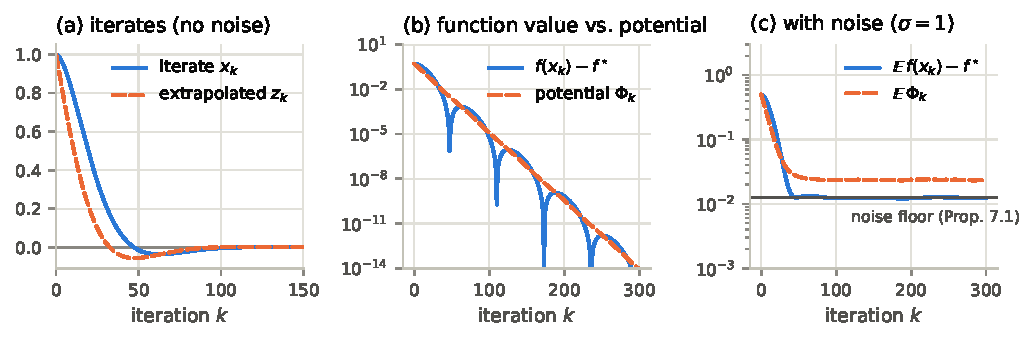
\includegraphics[width=\textwidth]{figures/potential.pdf}
\caption{Heavy ball on $f(x)=\frac12x^2$ ($L=1$) with $\beta=0.9$ and
$\alpha=(1-\beta)^2/(2L)=0.005$, the largest step allowed by \cref{thm:master}(b).
(a)~Without noise: the iterate $x_k$ and the extrapolated point $z_k$, which moves ahead
of $x_k$. (b)~Without noise: $f(x_k)-\fs$ is not monotone (it rises after each
overshoot), while the potential $\Phi_k$ of \cref{thm:master} decreases at every step.
(c)~With noise ($\sigma=1$, average over $20\,000$ runs): both expectations settle at a
noise floor; the floor of $\E f(x_k)$ agrees with the exact value of
\cref{prop:noise-floor} (horizontal line).}
\label{fig:potential}
\end{figure}

% ======================================================================
\section{The expected decrease inequality for SGDM}\label{sec:master}
% ======================================================================

We now carry out step \textbf{(T1)} of the template for SGDM. The plan has three steps:
(1)~run the SGD argument on the extrapolated points $z_k$, which do perform SGD steps
(\cref{lem:z}), and pay for the fact that the gradient is evaluated at the ``wrong'' point
$x_k$; (2)~show that the velocity, which controls this payment, is damped by friction;
(3)~combine the two in a potential.

\subsection{Step 1: descent at the extrapolated point}

\begin{lemma}[Descent at the extrapolated point]\label{lem:z-descent}
Under \cref{as:smooth,as:unbiased,as:variance}, for every $k\ge0$,
\begin{equation}\label{eq:z-descent}
  \Ek\bigl[f(z_{k+1})\bigr]\le f(z_k)-\frac\gamma2\,(1-L\gamma)\norm{\nabla f(x_k)}^2
  +\frac{L^2\gamma}{2}\norm{z_k-x_k}^2+\frac{L\gamma^2}{2}\sigma^2 .
\end{equation}
\end{lemma}

\begin{proof}
\emph{Descent lemma.} By \cref{lem:z}, $z_{k+1}=z_k-\gamma g_k$. Apply
\cref{lem:descent} with $x=z_k$ and $y=z_{k+1}$:
\[
  f(z_{k+1})\le f(z_k)-\gamma\ip{\nabla f(z_k)}{g_k}+\frac{L\gamma^2}{2}\norm{g_k}^2 .
\]
\emph{Conditional expectation.} The point $z_k$ is known at time $k$ (it is computed from
$x_k$ and $x_{k-1}$), hence so is $\nabla f(z_k)$. By \ref{R:mono}, \ref{R:known} and
\cref{as:unbiased}, $\Ek\ip{\nabla f(z_k)}{g_k}=\ip{\nabla f(z_k)}{\nabla f(x_k)}$, and by
\cref{lem:variance}, $\Ek\norm{g_k}^2\le\norm{\nabla f(x_k)}^2+\sigma^2$. Therefore
\[
  \Ek[f(z_{k+1})]\le f(z_k)-\gamma\ip{\nabla f(z_k)}{\nabla f(x_k)}
  +\frac{L\gamma^2}{2}\bigl(\norm{\nabla f(x_k)}^2+\sigma^2\bigr).
\]
\emph{The gradient is taken at the wrong point.} By polarization
(\cref{lem:elementary}(c)) with $a=\nabla f(z_k)$, $b=\nabla f(x_k)$, and then
$L$-smoothness,
\begin{align*}
  -\ip{\nabla f(z_k)}{\nabla f(x_k)}
  &=\tfrac12\norm{\nabla f(z_k)-\nabla f(x_k)}^2-\tfrac12\norm{\nabla f(z_k)}^2-\tfrac12\norm{\nabla f(x_k)}^2\\
  &\le\tfrac{L^2}{2}\norm{z_k-x_k}^2-\tfrac12\norm{\nabla f(x_k)}^2,
\end{align*}
where we also dropped $-\frac12\norm{\nabla f(z_k)}^2\le0$. Multiply by $\gamma$ and
insert into the previous display.
\end{proof}

Compared with SGD (\cref{lem:sgd-step}), the only new term is
$\frac{L^2\gamma}{2}\norm{z_k-x_k}^2$, the price of evaluating the gradient at $x_k$
instead of $z_k$. By \eqref{eq:z-minus-x} it equals
$\frac{L^2\gamma}{2}\bigl(\frac{\beta}{1-\beta}\bigr)^2\norm{v_k}^2$: it is
\emph{quadratic} in the velocity, hence of higher order in the step size than the
troublesome inertia term $\beta\ip{\nabla f(x_k)}{v_k}$ of \eqref{eq:naive}, which was
linear. This is what the change of variables $x_k\mapsto z_k$ buys.

\subsection{Step 2: friction damps the velocity}

\begin{lemma}[Velocity recursion]\label{lem:velocity}
Under \cref{as:unbiased,as:variance}, for every $k\ge0$,
\begin{equation}\label{eq:velocity-bound}
  \Ek\norm{v_{k+1}}^2\le\beta\norm{v_k}^2+(1-\beta)\gamma^2\norm{\nabla f(x_k)}^2+(1-\beta)^2\gamma^2\sigma^2 .
\end{equation}
\end{lemma}

\begin{proof}
By \eqref{eq:velocity}, $v_{k+1}=\beta v_k-\alpha g_k$. Since $v_k$ is known at time $k$,
its conditional mean is $\Ek[v_{k+1}]=\beta v_k-\alpha\nabla f(x_k)$ (rules \ref{R:lin},
\ref{R:known} and \cref{as:unbiased}), and $v_{k+1}-\Ek[v_{k+1}]=-\alpha\bigl(g_k-\nabla f(x_k)\bigr)$.
The variance decomposition (\cref{lem:variance}) and \cref{as:variance} give
\[
  \Ek\norm{v_{k+1}}^2=\norm{\beta v_k-\alpha\nabla f(x_k)}^2+\alpha^2\Ek\norm{g_k-\nabla f(x_k)}^2
  \le\norm{\beta v_k-\alpha\nabla f(x_k)}^2+\alpha^2\sigma^2 .
\]
Because $\alpha=(1-\beta)\gamma$, we can write
$\beta v_k-\alpha\nabla f(x_k)=\beta\,v_k+(1-\beta)\,\bigl(-\gamma\nabla f(x_k)\bigr)$, a convex
combination. By \cref{lem:elementary}(d) with $\theta=\beta$,
$\norm{\beta v_k-\alpha\nabla f(x_k)}^2\le\beta\norm{v_k}^2+(1-\beta)\gamma^2\norm{\nabla f(x_k)}^2$.
Finally $\alpha^2=(1-\beta)^2\gamma^2$.
\end{proof}

In words: each step, friction keeps only a fraction $\beta$ of the squared velocity, and the
gradient and the noise inject new velocity.

\subsection{Step 3: the potential and the main inequality}

\begin{tcolorbox}[keybox]
\begin{theorem}[Expected decrease for SGDM]\label{thm:master}
Let \cref{as:smooth,as:lower,as:unbiased,as:variance} hold, $\beta\in[0,1)$, $\alpha>0$,
$\gamma=\alpha/(1-\beta)$, and define
\begin{equation}\label{eq:potential}
  \Phi_k:=f(z_k)-\fs+\cb\norm{x_k-x_{k-1}}^2\;\ge0,\qquad \cb:=\frac{L\beta^2}{2(1-\beta)^2}.
\end{equation}
\begin{enumerate}[label=\textup{(\alph*)}]
\item For every $k\ge0$ (no condition on $\alpha$),
\begin{equation}\label{eq:master-general}
  \Ek[\Phi_{k+1}]\le\Phi_k
  -\frac\gamma2\Bigl(1-\frac{L\gamma\,(1-\beta+\beta^2)}{1-\beta}\Bigr)\norm{\nabla f(x_k)}^2
  -\cb\,(1-\beta-L\gamma)\norm{v_k}^2
  +\frac{1+\beta^2}{2}\,L\gamma^2\sigma^2 .
\end{equation}
\item If $\alpha\le\frac{(1-\beta)^2}{2L}$, equivalently $L\gamma\le\frac{1-\beta}{2}$, then
for every $k\ge0$,
\begin{equation}\label{eq:master}
  \Ek[\Phi_{k+1}]\le\Phi_k-\frac\gamma4\norm{\nabla f(x_k)}^2
  -\frac{L\beta^2}{4(1-\beta)}\norm{x_k-x_{k-1}}^2+L\gamma^2\sigma^2 .
\end{equation}
\end{enumerate}
\end{theorem}
\end{tcolorbox}

\begin{proof}
By \eqref{eq:z-minus-x},
$\frac{L^2\gamma}{2}\norm{z_k-x_k}^2=\frac{L^2\gamma}{2}\cdot\frac{\beta^2}{(1-\beta)^2}\norm{v_k}^2
=L\gamma\,\cb\norm{v_k}^2$. Subtracting $\fs$ from \cref{lem:z-descent} therefore gives
\begin{equation}\label{eq:pf-master-1}
  \Ek[f(z_{k+1})]-\fs\le f(z_k)-\fs-\frac\gamma2(1-L\gamma)\norm{\nabla f(x_k)}^2
  +L\gamma\,\cb\norm{v_k}^2+\frac{L\gamma^2}{2}\sigma^2 .
\end{equation}
Multiplying \cref{lem:velocity} by $\cb\ge0$ gives
\begin{equation}\label{eq:pf-master-2}
  \cb\,\Ek\norm{v_{k+1}}^2\le\cb\beta\norm{v_k}^2+\cb(1-\beta)\gamma^2\norm{\nabla f(x_k)}^2
  +\cb(1-\beta)^2\gamma^2\sigma^2 .
\end{equation}
By linearity \ref{R:lin}, the sum of the left-hand sides is $\Ek[\Phi_{k+1}]$. Adding
\eqref{eq:pf-master-1} and \eqref{eq:pf-master-2} and grouping terms,
\begin{align*}
  \Ek[\Phi_{k+1}]\le f(z_k)-\fs+\cb(\beta+L\gamma)\norm{v_k}^2
  &-\Bigl[\frac\gamma2(1-L\gamma)-\cb(1-\beta)\gamma^2\Bigr]\norm{\nabla f(x_k)}^2\\
  &+\Bigl[\frac{L\gamma^2}{2}+\cb(1-\beta)^2\gamma^2\Bigr]\sigma^2 .
\end{align*}
We simplify the three coefficients using $\cb=\frac{L\beta^2}{2(1-\beta)^2}$:
\begin{itemize}
\item \emph{velocity:} $\cb(\beta+L\gamma)=\cb-\cb(1-\beta-L\gamma)$, so
  $f(z_k)-\fs+\cb(\beta+L\gamma)\norm{v_k}^2=\Phi_k-\cb(1-\beta-L\gamma)\norm{v_k}^2$;
\item \emph{gradient:} $\cb(1-\beta)\gamma^2=\frac{L\beta^2\gamma^2}{2(1-\beta)}$, so the bracket equals
  $\frac\gamma2\bigl(1-L\gamma-\frac{L\gamma\beta^2}{1-\beta}\bigr)
  =\frac\gamma2\bigl(1-\frac{L\gamma(1-\beta+\beta^2)}{1-\beta}\bigr)$;
\item \emph{noise:} $\cb(1-\beta)^2\gamma^2=\frac{L\beta^2\gamma^2}{2}$, so the bracket equals
  $\frac{1+\beta^2}{2}L\gamma^2$.
\end{itemize}
This proves (a). For (b), assume $L\gamma\le\frac{1-\beta}{2}$. Then:
\begin{itemize}
\item $\frac{L\gamma(1-\beta+\beta^2)}{1-\beta}\le\frac{1-\beta+\beta^2}{2}\le\frac12$
  (because $\beta^2\le\beta$ for $\beta\in[0,1)$), so the gradient coefficient in (a) is at
  least $\frac\gamma2\cdot\frac12=\frac\gamma4$;
\item $1-\beta-L\gamma\ge\frac{1-\beta}2$, so
  $\cb(1-\beta-L\gamma)\ge\cb\frac{1-\beta}{2}=\frac{L\beta^2}{4(1-\beta)}$;
\item $\frac{1+\beta^2}{2}\le1$.
\end{itemize}
Inserting these three bounds into \eqref{eq:master-general} gives \eqref{eq:master}.
Finally, $\Phi_k\ge0$ because $f(z_k)\ge\fs$ (\cref{as:lower}).
\end{proof}

\subsection{Discussion}

\paragraph{Side by side with SGD.} \Cref{tab:side-by-side} compares
\cref{thm:master}(b) with \cref{lem:sgd-step}. The structure is identical; SGDM measures
progress with $\Phi_k$ instead of $f(x_k)-\fs$, and $\alpha$ is replaced by the effective
step size $\gamma$. Both quantities start at the same value, $\Phi_0=f(x_0)-\fs=\Dlt$,
because $v_0=0$ and $z_0=x_0$.

\begin{table}[ht]
\centering\small
\renewcommand{\arraystretch}{1.3}
\begin{tabular}{@{}lll@{}}
\toprule
 & SGD (\cref{lem:sgd-step}) & SGDM (\cref{thm:master}(b))\\
\midrule
measure of progress & $f(x_k)-\fs$ & $\Phi_k=f(z_k)-\fs+\cb\norm{x_k-x_{k-1}}^2$\\
step-size condition & $\alpha\le1/L$ & $\alpha\le(1-\beta)^2/(2L)$, i.e.\ $\gamma\le(1-\beta)/(2L)$\\
guaranteed progress & $\frac\alpha2\norm{\nabla f(x_k)}^2$ & $\frac\gamma4\norm{\nabla f(x_k)}^2$ (+ a velocity term)\\
price of noise & $\frac L2\alpha^2\sigma^2$ & $L\gamma^2\sigma^2$\\
value at $k=0$ & $\Dlt$ & $\Dlt$\\
\bottomrule
\end{tabular}
\caption{The expected decrease inequalities for SGD and SGDM.}
\label{tab:side-by-side}
\end{table}

\begin{tcolorbox}[intuition,title=Where the step-size condition comes from: an energy budget]
The potential contains a kinetic energy $\cb\norm{v_k}^2$. In each step friction removes
the fraction $1-\beta$ of it (\cref{lem:velocity} keeps only $\beta\norm{v_k}^2$), which
releases $\cb(1-\beta)\norm{v_k}^2$. Evaluating the gradient at the wrong point costs
$L\gamma\,\cb\norm{v_k}^2$ (\cref{lem:z-descent}). The budget balances exactly when
\[
  L\gamma<1-\beta\qquad\Longleftrightarrow\qquad\alpha<\frac{(1-\beta)^2}{L}:
\]
\emph{friction must dissipate kinetic energy faster than the gradient mismatch creates
error.} This is visible in \eqref{eq:master-general}: if $L\gamma<1-\beta$, both the
velocity coefficient and the gradient coefficient are positive (for the latter note that
$\frac{L\gamma(1-\beta+\beta^2)}{1-\beta}<1-\beta+\beta^2\le1$), so without noise
$\Phi_k$ strictly decreases until $x_k$ is stationary with zero velocity. Condition (b)
keeps half of the friction as a safety margin, which produces the clean constants. As
$\beta\to1$ the friction vanishes, and so does the admissible step.
\end{tcolorbox}

\begin{remark}[The case $\beta=0$]
For $\beta=0$ we have $\cb=0$, $z_k=x_k$, $\Phi_k=f(x_k)-\fs$, and
\eqref{eq:master-general} reads
$\Ek[f(x_{k+1})]\le f(x_k)-\frac\gamma2(1-L\gamma)\norm{\nabla f(x_k)}^2+\frac{L\gamma^2}{2}\sigma^2$:
this is \cref{lem:sgd-step} with a progress term smaller by about a factor $2$, the price of
discarding $-\frac12\norm{\nabla f(z_k)}^2$ in the polarization step. Constants in this
report are chosen for simplicity and are not optimized.
\end{remark}

\begin{remark}[Why both parts of the potential are needed]
Without the kinetic term, \eqref{eq:pf-master-1} leaves a positive term
$L\gamma\cb\norm{v_k}^2$ that $f(z_k)$ cannot absorb; adding $\cb\norm{v_k}^2$ and
\cref{lem:velocity} turns it into a decrease. Conversely, a potential built on $f(x_k)$
instead of $f(z_k)$ must absorb the first-order inertia term of \eqref{eq:naive}; this works
without noise (\cref{prop:energy}) but not with noise (\cref{rem:energy-noise}).
\end{remark}

\begin{corollary}[When does one step decrease the potential?]\label{cor:when-decrease}
Under the assumptions of \cref{thm:master}(b), $\Ek[\Phi_{k+1}]<\Phi_k$ whenever
\[
  \frac\gamma4\norm{\nabla f(x_k)}^2+\frac{L\beta^2}{4(1-\beta)}\norm{x_k-x_{k-1}}^2>L\gamma^2\sigma^2,
  \qquad\text{in particular whenever}\qquad \norm{\nabla f(x_k)}^2>4L\gamma\sigma^2 .
\]
Without noise ($\sigma=0$), $\Phi_k$ is non-increasing along every trajectory.
For comparison, SGD with $\alpha\le1/L$ decreases $f$ in expectation whenever
$\norm{\nabla f(x_k)}^2>L\alpha\sigma^2$.
\end{corollary}

\begin{proof}
Immediate from \eqref{eq:master} (and from \cref{lem:sgd-step} for SGD).
\end{proof}

So the circumstances under which SGDM makes progress \emph{in a single step} are the same
as for SGD: the signal $\norm{\nabla f(x_k)}^2$ must exceed the noise level, here
$4L\gamma\sigma^2$; outside this ``noise region'' the potential decreases in expectation,
inside it the noise can push it up. Shrinking $\gamma$ shrinks the noise region.

The potential also controls the function value at the actual iterate:

\begin{lemma}[The potential controls $f(x_k)$]\label{lem:phi-controls-f}
Under \cref{as:smooth,as:lower}, for all $x,z\in\R^d$,
\begin{equation}\label{eq:f-two-points}
  f(x)-\fs\le2\bigl(f(z)-\fs\bigr)+L\norm{x-z}^2 .
\end{equation}
Consequently the SGDM iterates satisfy $f(x_k)-\fs\le2\,\Phi_k$ for all $k\ge0$.
\end{lemma}

\begin{proof}
By the descent lemma with base point $z$, and Young's inequality
(\cref{lem:elementary}(b) with $\rho=1/L$),
\[
  f(x)\le f(z)+\ip{\nabla f(z)}{x-z}+\frac L2\norm{x-z}^2
  \le f(z)+\frac{1}{2L}\norm{\nabla f(z)}^2+L\norm{x-z}^2 .
\]
By \cref{lem:grad-gap}, $\frac1{2L}\norm{\nabla f(z)}^2\le f(z)-\fs$; subtracting $\fs$
gives \eqref{eq:f-two-points}. For the iterates take $x=x_k$, $z=z_k$: by
\eqref{eq:z-minus-x}, $L\norm{x_k-z_k}^2=\frac{L\beta^2}{(1-\beta)^2}\norm{v_k}^2=2\cb\norm{v_k}^2$,
so $f(x_k)-\fs\le2(f(z_k)-\fs)+2\cb\norm{v_k}^2=2\Phi_k$.
\end{proof}

Without noise and under \cref{thm:master}(b), this gives $f(x_k)-\fs\le2\Phi_k\le2\Phi_0=2\Dlt$:
the function value may go up (\cref{fig:potential}(b)), but never above
$\fs+2\bigl(f(x_0)-\fs\bigr)$.

\begin{remark}[Two extensions]\label{rem:extensions}
\begin{enumerate}[label=\textup{(\roman*)},leftmargin=2em]
\item \emph{Varying step sizes.} Suppose Algorithm~1 uses $\alpha_k$ at iteration $k$
  (heavy-ball form) and set $\gamma_k=\alpha_k/(1-\beta)$. Each ingredient of the proof of
  \cref{thm:master} is a statement about a single iteration---\cref{lem:z} holds with
  $\gamma_k$ by \cref{rem:varying}, and \cref{lem:z-descent,lem:velocity} only involve
  step $k$---and the weight $\cb$ does not depend on the step size. Hence
  \eqref{eq:master} holds at iteration $k$ with $\gamma_k$ in place of $\gamma$ whenever
  $L\gamma_k\le\frac{1-\beta}{2}$, with the \emph{same} potential $\Phi_k$.
\item \emph{Noise that grows with the gradient.} If \cref{as:variance} is replaced by
  $\Ek\norm{g_k-\nabla f(x_k)}^2\le\sigma^2+M\norm{\nabla f(x_k)}^2$ for some $M\ge0$, then
  \eqref{eq:master} still holds provided $\alpha\le\frac{(1-\beta)^2}{2L(1+M)}$. Indeed,
  the only changes in the proof are $\Ek\norm{g_k}^2\le(1+M)\norm{\nabla f(x_k)}^2+\sigma^2$
  in \cref{lem:z-descent} and an extra $\alpha^2M\norm{\nabla f(x_k)}^2$ in
  \cref{lem:velocity}; the gradient coefficient becomes
  $\frac\gamma2\bigl[1-L\gamma(1+M)-\frac{L\gamma\beta^2}{1-\beta}(1+(1-\beta)M)\bigr]
  \ge\frac\gamma2\bigl[1-\frac{1-\beta}{2}-\frac{\beta^2}{2}\bigr]\ge\frac\gamma4$ when
  $L\gamma(1+M)\le\frac{1-\beta}{2}$, and the other coefficients are unchanged.
\end{enumerate}
\end{remark}

% ======================================================================
\section{Convergence theorems for SGDM}\label{sec:convergence}
% ======================================================================

With \cref{thm:master} in hand, steps \textbf{(T2)}--\textbf{(T3)} of the template
(\cref{sec:template}) go through essentially verbatim. Recall $\Dlt=f(x_0)-\fs$ and
$\gamma=\alpha/(1-\beta)$.

\subsection{Nonconvex functions, constant step size}

\begin{tcolorbox}[keybox]
\begin{theorem}[SGDM, nonconvex]\label{thm:nonconvex}
Let \cref{as:smooth,as:lower,as:unbiased,as:variance} hold, $\beta\in[0,1)$ and
$0<\alpha\le\frac{(1-\beta)^2}{2L}$. Then for every $K\ge1$,
\begin{equation}\label{eq:nonconvex}
  \frac1K\sum_{k=0}^{K-1}\E\norm{\nabla f(x_k)}^2\le\frac{4\Dlt}{\gamma K}+4L\gamma\sigma^2 .
\end{equation}
\end{theorem}
\end{tcolorbox}

\begin{proof}
Drop the (non-positive) velocity term in \eqref{eq:master} and take full expectations
(tower property \ref{R:tower}):
$\E\Phi_{k+1}\le\E\Phi_k-\frac\gamma4\E\norm{\nabla f(x_k)}^2+L\gamma^2\sigma^2$.
Summing over $k=0,\dots,K-1$, the potentials telescope:
\[
  \E\Phi_K\le\Phi_0-\frac\gamma4\sum_{k=0}^{K-1}\E\norm{\nabla f(x_k)}^2+KL\gamma^2\sigma^2 .
\]
Now $\Phi_0=f(z_0)-\fs+\cb\norm{v_0}^2=f(x_0)-\fs=\Dlt$ and $\E\Phi_K\ge0$. Rearranging,
$\frac\gamma4\sum_{k<K}\E\norm{\nabla f(x_k)}^2\le\Dlt+KL\gamma^2\sigma^2$; divide by $\gamma K/4$.
\end{proof}

Since a minimum never exceeds an average, \eqref{eq:nonconvex} also bounds
$\min_{k<K}\E\norm{\nabla f(x_k)}^2$. In practice one can output $x_R$ with $R$ drawn
uniformly from $\{0,\dots,K-1\}$, independently of everything else; then
$\E\norm{\nabla f(x_R)}^2$ equals the left-hand side of \eqref{eq:nonconvex}~\cite{ghadimilan2013}.

\begin{corollary}[Step size and iteration complexity]\label{cor:rate}
Under the assumptions of \cref{thm:nonconvex}, fix $K\ge1$ and choose
\[
  \gamma=\min\Bigl\{\frac{1-\beta}{2L},\;\frac1\sigma\sqrt{\frac{\Dlt}{LK}}\Bigr\}
  \quad\Bigl(\gamma=\tfrac{1-\beta}{2L}\text{ if }\sigma=0\Bigr),
  \qquad\alpha=(1-\beta)\gamma .
\]
Then
\begin{equation}\label{eq:rate}
  \frac1K\sum_{k=0}^{K-1}\E\norm{\nabla f(x_k)}^2\le\frac{8L\Dlt}{(1-\beta)K}+8\sigma\sqrt{\frac{L\Dlt}{K}} .
\end{equation}
Consequently $\min_{k<K}\E\norm{\nabla f(x_k)}^2\le\eps^2$ as soon as
$K\ge\max\bigl\{\frac{16L\Dlt}{(1-\beta)\eps^2},\,\frac{256L\Dlt\sigma^2}{\eps^4}\bigr\}$.
\end{corollary}

\begin{proof}
The chosen $\gamma$ satisfies $L\gamma\le\frac{1-\beta}2$, so \cref{thm:nonconvex}
applies. Using $\frac{1}{\min\{a,b\}}\le\frac1a+\frac1b$ for $a,b>0$,
\[
  \frac{4\Dlt}{\gamma K}\le\frac{4\Dlt}{K}\Bigl(\frac{2L}{1-\beta}+\sigma\sqrt{\frac{LK}{\Dlt}}\Bigr)
  =\frac{8L\Dlt}{(1-\beta)K}+4\sigma\sqrt{\frac{L\Dlt}{K}},
  \qquad
  4L\gamma\sigma^2\le4L\sigma^2\cdot\frac1\sigma\sqrt{\frac{\Dlt}{LK}}=4\sigma\sqrt{\frac{L\Dlt}{K}} .
\]
Adding gives \eqref{eq:rate}. For the complexity statement, each of the two terms in
\eqref{eq:rate} is at most $\eps^2/2$ under the stated condition on $K$.
\end{proof}

\paragraph{Comparison with SGD.} For SGD the analogous choice gives
$\frac{2L\Dlt}{K}+2\sigma\sqrt{\frac{2L\Dlt}{K}}$ (\cref{sec:sgd}). The dominant term for
large $K$ (or small $\eps$), of order $\sigma\sqrt{L\Dlt/K}$, is the same for SGD and SGDM
up to a constant: \emph{in the worst case momentum neither improves nor degrades the
asymptotic rate.} Momentum costs a factor $1/(1-\beta)$ in the noise-free term, which
reflects the more conservative step-size condition.

\begin{corollary}[Exact gradients]\label{cor:deterministic}
Let \cref{as:smooth,as:lower} hold, $\sigma=0$ (that is, $g_k=\nabla f(x_k)$), $\beta\in[0,1)$
and $\alpha=\frac{(1-\beta)^2}{2L}$. Then
\begin{enumerate}[label=\textup{(\roman*)}]
\item $\Phi_{k+1}\le\Phi_k$ for all $k$, and $f(x_k)\le\fs+2\Dlt$ for all $k$;
\item $\sum_{k=0}^\infty\norm{\nabla f(x_k)}^2\le\frac{8L\Dlt}{1-\beta}$; in particular $\nabla f(x_k)\to0$;
\item $\min_{0\le k<K}\norm{\nabla f(x_k)}^2\le\frac{8L\Dlt}{(1-\beta)K}$.
\end{enumerate}
\end{corollary}

\begin{proof}
Without noise everything is deterministic, and \eqref{eq:master} with
$\gamma=\frac{1-\beta}{2L}$ reads $\Phi_{k+1}\le\Phi_k-\frac\gamma4\norm{\nabla f(x_k)}^2$.
(i) follows, together with $f(x_k)-\fs\le2\Phi_k\le2\Phi_0=2\Dlt$
(\cref{lem:phi-controls-f}). (ii) Summing, $\frac\gamma4\sum_{k<K}\norm{\nabla f(x_k)}^2\le\Phi_0-\Phi_K\le\Dlt$
for every $K$, so the series converges with sum at most $4\Dlt/\gamma=8L\Dlt/(1-\beta)$, and its
terms tend to zero. (iii) The minimum is at most the average, $\frac1K\cdot\frac{8L\Dlt}{1-\beta}$.
\end{proof}

\subsection{Nonconvex functions, diminishing step sizes}

\begin{theorem}[SGDM with diminishing steps]\label{thm:diminishing}
Let \cref{as:smooth,as:lower,as:unbiased,as:variance} hold and $\beta\in[0,1)$. Run
Algorithm~1 in heavy-ball form with step size $\alpha_k$ at iteration $k$,
$x_{k+1}=x_k-\alpha_kg_k+\beta(x_k-x_{k-1})$, where $\gamma_k:=\alpha_k/(1-\beta)$ satisfies
$0<\gamma_k\le\frac{1-\beta}{2L}$ for all $k$. Then for every $K\ge1$,
\begin{equation}\label{eq:diminishing}
  \sum_{k=0}^{K-1}\gamma_k\,\E\norm{\nabla f(x_k)}^2\le4\Dlt+4L\sigma^2\sum_{k=0}^{K-1}\gamma_k^2 .
\end{equation}
Consequently:
\begin{enumerate}[label=\textup{(\alph*)}]
\item $\displaystyle\min_{0\le k<K}\E\norm{\nabla f(x_k)}^2\le
       \frac{4\Dlt+4L\sigma^2\sum_{k<K}\gamma_k^2}{\sum_{k<K}\gamma_k}$.
\item \emph{(Robbins--Monro steps.)} If $\sum_k\gamma_k=\infty$ and $\sum_k\gamma_k^2<\infty$,
  then $\min_{k<K}\E\norm{\nabla f(x_k)}^2\to0$ as $K\to\infty$ and
  $\liminf_{k\to\infty}\E\norm{\nabla f(x_k)}^2=0$. Moreover, with probability one,
  $\sum_k\gamma_k\norm{\nabla f(x_k)}^2<\infty$ and $\liminf_{k\to\infty}\norm{\nabla f(x_k)}=0$.
\item If $\gamma_k=\gamma_0/\sqrt{k+1}$ with $\gamma_0\le\frac{1-\beta}{2L}$, then
  $\displaystyle\min_{0\le k<K}\E\norm{\nabla f(x_k)}^2\le\frac{4\Dlt+4L\sigma^2\gamma_0^2(1+\ln K)}{\gamma_0\sqrt K}
  =O\Bigl(\frac{\log K}{\sqrt K}\Bigr)$.
\end{enumerate}
\end{theorem}

\begin{proof}
By \cref{rem:extensions}(i), inequality \eqref{eq:master} holds at every iteration with
$\gamma_k$: $\Ek\Phi_{k+1}\le\Phi_k-\frac{\gamma_k}4\norm{\nabla f(x_k)}^2+L\gamma_k^2\sigma^2$.
Taking expectations, summing over $k<K$, and using $\Phi_0=\Dlt$ and $\E\Phi_K\ge0$ gives
$\frac14\sum_{k<K}\gamma_k\E\norm{\nabla f(x_k)}^2\le\Dlt+L\sigma^2\sum_{k<K}\gamma_k^2$,
which is \eqref{eq:diminishing}.

(a) The left side of \eqref{eq:diminishing} is at least
$\bigl(\min_{k<K}\E\norm{\nabla f(x_k)}^2\bigr)\sum_{k<K}\gamma_k$.

(b) Let $C:=4\Dlt+4L\sigma^2\sum_{k=0}^\infty\gamma_k^2<\infty$. By (a),
$\min_{k<K}\E\norm{\nabla f(x_k)}^2\le C/\sum_{k<K}\gamma_k\to0$. If
$\liminf_k\E\norm{\nabla f(x_k)}^2$ were positive, there would be $\eps>0$ and $k_0$ with
$\E\norm{\nabla f(x_k)}^2\ge\eps$ for all $k\ge k_0$, and then the left side of
\eqref{eq:diminishing} would be at least $\eps\sum_{k_0\le k<K}\gamma_k\to\infty$,
contradicting the bound $C$. For the almost-sure statement, the random variables
$S_K:=\sum_{k<K}\gamma_k\norm{\nabla f(x_k)}^2$ are non-negative and non-decreasing in
$K$, so $S_\infty:=\lim_KS_K\in[0,\infty]$ exists, and by the monotone convergence
theorem $\E S_\infty=\lim_K\E S_K\le C<\infty$. A non-negative random variable with finite
expectation is finite with probability one, so $S_\infty<\infty$ almost surely. On this
event $\liminf_k\norm{\nabla f(x_k)}=0$: otherwise $\norm{\nabla f(x_k)}^2\ge\eps$ for some
$\eps>0$ and all large $k$, which would force $S_\infty=\infty$ because $\sum_k\gamma_k=\infty$.

(c) $\sum_{k<K}\gamma_k=\gamma_0\sum_{j=1}^Kj^{-1/2}\ge\gamma_0\sqrt K$, since each of the
$K$ terms is at least $K^{-1/2}$; and
$\sum_{k<K}\gamma_k^2=\gamma_0^2\sum_{j=1}^K\frac1j\le\gamma_0^2\bigl(1+\int_1^K\frac{dt}{t}\bigr)=\gamma_0^2(1+\ln K)$.
Insert both into (a).
\end{proof}

Step sizes such as $\gamma_k=\gamma_0/(k+1)^{0.6}$ satisfy the Robbins--Monro
conditions~\cite{robbins1951}. Stronger almost-sure statements (a limit rather than a
$\liminf$) are known for SGD~\cite{bertsekas2000} and for the stochastic heavy-ball
method~\cite{gadat2018,sebbouh2021}; they require more advanced martingale tools such as
the Robbins--Siegmund theorem~\cite{robbinssiegmund1971}.

\subsection{Functions satisfying the PL inequality}

\begin{lemma}\label{lem:phi-pl}
Under \cref{as:smooth,as:lower} and the PL inequality \eqref{eq:pl}, the SGDM iterates satisfy
\[
  \Phi_k\le\frac1\mu\norm{\nabla f(x_k)}^2+3\cb\norm{x_k-x_{k-1}}^2\qquad\text{for all }k\ge0.
\]
\end{lemma}

\begin{proof}
If $\nabla f\equiv0$ then $f$ is constant, $\Phi_k=\cb\norm{v_k}^2$, and there is nothing to
prove; otherwise $\mu\le L$ by \cref{lem:pl-facts}(b). Write
$f(z_k)-\fs=\bigl(f(z_k)-f(x_k)\bigr)+\bigl(f(x_k)-\fs\bigr)$. By the descent lemma and Young's
inequality with $\rho=1/L$,
$f(z_k)-f(x_k)\le\ip{\nabla f(x_k)}{z_k-x_k}+\frac L2\norm{z_k-x_k}^2
\le\frac1{2L}\norm{\nabla f(x_k)}^2+L\norm{z_k-x_k}^2$, and by PL,
$f(x_k)-\fs\le\frac1{2\mu}\norm{\nabla f(x_k)}^2$. Since $\frac1{2L}+\frac1{2\mu}\le\frac1\mu$
and $L\norm{z_k-x_k}^2=2\cb\norm{v_k}^2$ (see the proof of \cref{lem:phi-controls-f}),
$f(z_k)-\fs\le\frac1\mu\norm{\nabla f(x_k)}^2+2\cb\norm{v_k}^2$. Add $\cb\norm{v_k}^2$.
\end{proof}

\begin{tcolorbox}[keybox]
\begin{theorem}[SGDM under the PL inequality]\label{thm:pl}
Let \cref{as:smooth,as:lower,as:unbiased,as:variance} and the PL inequality \eqref{eq:pl}
hold, $\beta\in[0,1)$ and $0<\alpha\le\frac{(1-\beta)^2}{2L}$. Then for all $k\ge0$,
\[
  \E\Phi_k\le\Bigl(1-\frac{\gamma\mu}{4}\Bigr)^k\Dlt+\frac{4L\gamma\sigma^2}{\mu},
  \qquad
  \E f(x_k)-\fs\le2\Bigl(1-\frac{\gamma\mu}{4}\Bigr)^k\Dlt+\frac{8L\gamma\sigma^2}{\mu}.
\]
\end{theorem}
\end{tcolorbox}

\begin{proof}
Since $\frac{L\beta^2}{4(1-\beta)}=\frac{\cb(1-\beta)}{2}$, \eqref{eq:master} reads
\[
  \Ek\Phi_{k+1}\le\Phi_k-\Bigl[\frac\gamma4\norm{\nabla f(x_k)}^2+\frac{\cb(1-\beta)}{2}\norm{v_k}^2\Bigr]
  +L\gamma^2\sigma^2 .
\]
By \cref{lem:phi-pl}, $\frac{\gamma\mu}{4}\Phi_k\le\frac\gamma4\norm{\nabla f(x_k)}^2+\frac{3\gamma\mu}{4}\cb\norm{v_k}^2$,
and $\frac{3\gamma\mu}{4}\cb\le\frac{\cb(1-\beta)}{2}$ because
$\gamma\mu\le\gamma L\le\frac{1-\beta}{2}\le\frac{2(1-\beta)}{3}$. Hence the bracket is at
least $\frac{\gamma\mu}4\Phi_k$, and
\begin{equation}\label{eq:pl-contraction}
  \Ek\Phi_{k+1}\le\Bigl(1-\frac{\gamma\mu}4\Bigr)\Phi_k+L\gamma^2\sigma^2 .
\end{equation}
Note $0<\frac{\gamma\mu}{4}\le\frac18$. Taking expectations and unrolling as in the proof of
\cref{thm:sgd-pl},
$\E\Phi_k\le(1-\frac{\gamma\mu}4)^k\Phi_0+L\gamma^2\sigma^2\sum_{j<k}(1-\frac{\gamma\mu}4)^j
\le(1-\frac{\gamma\mu}4)^k\Dlt+L\gamma^2\sigma^2\cdot\frac4{\gamma\mu}$. The bound on
$f(x_k)$ follows from $f(x_k)-\fs\le2\Phi_k$ (\cref{lem:phi-controls-f}).
\end{proof}

Compared with SGD (\cref{thm:sgd-pl}: contraction $1-\alpha\mu$, floor
$\frac{L\alpha\sigma^2}{2\mu}$), the statement has the same form with $\alpha$ replaced by
$\gamma$ and worse constants. With the largest admissible step,
$\gamma=\frac{1-\beta}{2L}$, the contraction factor is $1-\frac{(1-\beta)\mu}{8L}$: \emph{in
this worst-case analysis momentum does not accelerate} (see \cref{sec:momentum-help}).

\begin{corollary}[PL inequality, decreasing steps]\label{cor:pl-decay}
Under the assumptions of \cref{thm:pl} (except for the step size), run Algorithm~1 in
heavy-ball form with $\gamma_k=\frac{8}{\mu(k+a)}$, $\alpha_k=(1-\beta)\gamma_k$, where
$a\ge\frac{16L}{\mu(1-\beta)}$. Then for all $k\ge0$,
\[
  \E\Phi_k\le\frac{\nu}{k+a},\qquad\E f(x_k)-\fs\le\frac{2\nu}{k+a},\qquad
  \nu:=\max\Bigl\{a\Dlt,\;\frac{64L\sigma^2}{\mu^2}\Bigr\}.
\]
\end{corollary}

\begin{proof}
Since $\gamma_k\le\gamma_0=\frac{8}{\mu a}\le\frac{1-\beta}{2L}$, the one-step contraction
\eqref{eq:pl-contraction} holds at every iteration with $\gamma_k$ (its proof uses only
\eqref{eq:master} at iteration $k$, valid by \cref{rem:extensions}(i), and
\cref{lem:phi-pl}). With $e_k:=\E\Phi_k$ and $\frac{\gamma_k\mu}{4}=\frac2{k+a}$,
\[
  e_{k+1}\le\Bigl(1-\frac{2}{k+a}\Bigr)e_k+\frac{64L\sigma^2}{\mu^2(k+a)^2}.
\]
We show $e_k\le\nu/(k+a)$ by induction. For $k=0$, $e_0=\Dlt\le\nu/a$. If
$e_k\le\nu/(k+a)$, then, because $1-\frac2{k+a}\ge0$ (note $a\ge16$) and
$\frac{64L\sigma^2}{\mu^2}\le\nu$,
\[
  e_{k+1}\le\frac{(k+a-2)\,\nu}{(k+a)^2}+\frac{\nu}{(k+a)^2}=\frac{(k+a-1)\,\nu}{(k+a)^2}\le\frac{\nu}{k+a+1},
\]
where the last step uses $(k+a-1)(k+a+1)=(k+a)^2-1\le(k+a)^2$. The bound on $f(x_k)$ follows
from \cref{lem:phi-controls-f}.
\end{proof}

\subsection{Convex functions}

For convex functions a different potential---a distance to the minimizer, as in the
classical convex analysis of SGD---gives a guarantee under a step-size condition that
does not degrade as $\beta\to1$.

\begin{tcolorbox}[keybox]
\begin{theorem}[SGDM, convex]\label{thm:convex}
Let \cref{as:smooth,as:unbiased,as:variance} hold, let $f$ be convex with a minimizer
$x^\star$ (so $\fs=f(x^\star)$), $\beta\in[0,1)$, and $0<\alpha\le\frac{1-\beta}{2L}$, i.e.\
$L\gamma\le\frac12$. Define
\[
  \Psi_k:=\norm{z_k-x^\star}^2+\frac{2\gamma\beta}{1-\beta}\bigl(f(x_{k-1})-\fs\bigr)\;\ge0 .
\]
\begin{enumerate}[label=\textup{(\alph*)}]
\item For every $k\ge0$:
  $\Ek\Psi_{k+1}\le\Psi_k-2\gamma(1-L\gamma)\bigl(f(x_k)-\fs\bigr)+\gamma^2\sigma^2
  \le\Psi_k-\gamma\bigl(f(x_k)-\fs\bigr)+\gamma^2\sigma^2$.
\item For every $K\ge1$, with $\bar x_K:=\frac1K\sum_{k<K}x_k$,
  \[
    \E f(\bar x_K)-\fs\le\frac1K\sum_{k=0}^{K-1}\bigl(\E f(x_k)-\fs\bigr)
    \le\frac{\norm{x_0-x^\star}^2}{\gamma K}+\frac{2\beta\Dlt}{(1-\beta)K}+\gamma\sigma^2 .
  \]
\item With $D:=\norm{x_0-x^\star}$ and $\gamma=\min\{\frac1{2L},\frac{D}{\sigma\sqrt K}\}$:
  $\E f(\bar x_K)-\fs\le\frac{2LD^2}{K}+\frac{2\beta\Dlt}{(1-\beta)K}+\frac{2\sigma D}{\sqrt K}$.
\end{enumerate}
\end{theorem}
\end{tcolorbox}

\begin{proof}
(a) By \cref{lem:z}, $z_{k+1}-x^\star=(z_k-x^\star)-\gamma g_k$, hence
$\norm{z_{k+1}-x^\star}^2=\norm{z_k-x^\star}^2-2\gamma\ip{g_k}{z_k-x^\star}+\gamma^2\norm{g_k}^2$.
Taking $\Ek$ ($z_k$ is known at time $k$; \cref{as:unbiased}; \cref{lem:variance}):
\[
  \Ek\norm{z_{k+1}-x^\star}^2\le\norm{z_k-x^\star}^2-2\gamma\ip{\nabla f(x_k)}{z_k-x^\star}
  +\gamma^2\bigl(\norm{\nabla f(x_k)}^2+\sigma^2\bigr).
\]
Split $z_k-x^\star=(x_k-x^\star)+\frac{\beta}{1-\beta}(x_k-x_{k-1})$ and use convexity
(\cref{def:convex}) twice: with $y=x^\star$,
$\ip{\nabla f(x_k)}{x_k-x^\star}\ge f(x_k)-\fs$; with $y=x_{k-1}$,
$\ip{\nabla f(x_k)}{x_k-x_{k-1}}\ge f(x_k)-f(x_{k-1})$. Together with
$\norm{\nabla f(x_k)}^2\le2L(f(x_k)-\fs)$ (\cref{lem:grad-gap}) this yields
\[
  \Ek\norm{z_{k+1}-x^\star}^2\le\norm{z_k-x^\star}^2-2\gamma(1-L\gamma)\bigl(f(x_k)-\fs\bigr)
  +\frac{2\gamma\beta}{1-\beta}\bigl(f(x_{k-1})-f(x_k)\bigr)+\gamma^2\sigma^2 .
\]
Add $\frac{2\gamma\beta}{1-\beta}(f(x_k)-\fs)$, which is known at time $k$, to both
sides. The left side becomes $\Ek\Psi_{k+1}$ and the right side becomes
$\Psi_k-2\gamma(1-L\gamma)(f(x_k)-\fs)+\gamma^2\sigma^2$. Finally $L\gamma\le\frac12$ gives
$2\gamma(1-L\gamma)\ge\gamma$.

(b) Take expectations in (a) and sum over $k<K$:
$\E\Psi_K\le\Psi_0-\gamma\sum_{k<K}(\E f(x_k)-\fs)+K\gamma^2\sigma^2$, where
$\Psi_0=\norm{x_0-x^\star}^2+\frac{2\gamma\beta}{1-\beta}\Dlt$ (recall $z_0=x_0=x_{-1}$) and
$\E\Psi_K\ge0$. Rearrange and divide by $\gamma K$. The first inequality is Jensen's
inequality: by convexity, $f(x_k)\ge f(\bar x_K)+\ip{\nabla f(\bar x_K)}{x_k-\bar x_K}$
for each $k$, and averaging over $k$ the inner products cancel.

(c) As in \cref{cor:rate}: $\frac{D^2}{\gamma K}\le\frac{D^2}{K}\bigl(2L+\frac{\sigma\sqrt K}{D}\bigr)$ and
$\gamma\sigma^2\le\frac{\sigma D}{\sqrt K}$.
\end{proof}

\begin{remark}[Why convexity relaxes the step-size condition]
In the convex case the step-size restriction $L\gamma\le\frac12$ does not depend on
$\beta$---it is the SGD condition with $\alpha$ replaced by $\gamma$---whereas the
nonconvex analysis needs $L\gamma\le\frac{1-\beta}2$. Convexity lets us bound the
troublesome inner product $\ip{\nabla f(x_k)}{x_k-x_{k-1}}$ by a difference of function
values, which telescopes, instead of paying for it with kinetic energy. The extra term
$\frac{2\beta\Dlt}{(1-\beta)K}$ is the price of momentum; since $\Dlt\le\frac L2D^2$ (descent
lemma at $x^\star$, where $\nabla f(x^\star)=0$), it is at most
$\frac{\beta}{1-\beta}\cdot\frac{LD^2}{K}$.
\end{remark}

% ======================================================================
\section{Under what circumstances does SGDM converge?}\label{sec:circumstances}
% ======================================================================

The theorems of \cref{sec:convergence} hold under explicit \emph{sufficient} conditions.
This section asks which parts of these conditions can be removed, what goes wrong when
they fail, and how they fit together. Quadratic functions, for which everything can be
computed exactly, serve as test cases.

\subsection{A constant step size leaves a noise floor}

All constant-step results contain a term proportional to $\gamma\sigma^2$ that does not
vanish as $K\to\infty$. The next proposition shows that this is not an artifact of the
proofs: the floor is real, of exactly this order, and the same for SGD and SGDM at equal
effective step size.

\begin{proposition}[Exact noise floor on a quadratic]\label{prop:noise-floor}
Let $f(x)=\frac h2x^2$ on $\R$ with $h>0$, and let $g_k=hx_k+\xi_k$, where
$\xi_0,\xi_1,\dots$ are independent with $\E\xi_k=0$ and $\E\xi_k^2=\sigma^2$ (so
\cref{as:smooth,as:lower,as:unbiased,as:variance} hold with $L=h$). Let $\beta\in[0,1)$ and
$0<\alpha h<2(1+\beta)$. Then, for every starting point $x_0$,
\begin{equation}\label{eq:noise-floor}
  \lim_{k\to\infty}\E f(x_k)=\frac{\gamma\sigma^2}{2}\cdot\frac{1+\beta}{2(1+\beta)-\alpha h},
  \qquad
  \lim_{k\to\infty}\E\bigl[f'(x_k)^2\bigr]=h\gamma\sigma^2\cdot\frac{1+\beta}{2(1+\beta)-\alpha h}.
\end{equation}
In particular $\lim_k\E f(x_k)\ge\frac{\gamma\sigma^2}{4}$, and
$\lim_k\E f(x_k)=\frac{\gamma\sigma^2}{4}+\frac{\gamma\sigma^2}{4}\cdot\frac{\alpha h}{2(1+\beta)-\alpha h}$,
so to first order the floor depends on $(\alpha,\beta)$ only through $\gamma=\alpha/(1-\beta)$.
\end{proposition}

\begin{proof}
Let $a:=1+\beta-\alpha h$; the update reads $x_{k+1}=ax_k-\beta x_{k-1}-\alpha\xi_k$. With
$X_k:=(x_k,x_{k-1})^\top$ (and $x_{-1}=x_0$),
\[
  X_{k+1}=MX_k+w_k,\qquad M:=\begin{pmatrix}a&-\beta\\1&0\end{pmatrix},\qquad
  w_k:=\begin{pmatrix}-\alpha\xi_k\\0\end{pmatrix}.
\]
\emph{Second moments.} Let $C_k:=\E[X_kX_k^\top]$, a symmetric $2\times2$ matrix whose
$(1,1)$ entry is $\E x_k^2$. Since $X_k$ is a function of $\xi_0,\dots,\xi_{k-1}$, it is
independent of $\xi_k$, so $\E[X_kw_k^\top]=\E[X_k]\,\E[w_k]^\top=0$. Expanding the product,
\[
  C_{k+1}=\E\bigl[(MX_k+w_k)(MX_k+w_k)^\top\bigr]=MC_kM^\top+Q,\qquad
  Q:=\E[w_kw_k^\top]=\begin{pmatrix}\alpha^2\sigma^2&0\\0&0\end{pmatrix},
\]
and by induction $C_k=M^kC_0(M^\top)^k+\sum_{j=0}^{k-1}M^jQ(M^\top)^j$.

\emph{Convergence.} The eigenvalues of $M$ are the roots of
$\det(\lambda I-M)=\lambda^2-a\lambda+\beta$. By the proof of
\cref{prop:quadratic-stability} below, the assumption $0<\alpha h<2(1+\beta)$ implies that
both roots have modulus less than one. Then the entries of $M^k$ tend to zero
geometrically fast (\cref{lem:matrix-powers} in the appendix), so
$M^kC_0(M^\top)^k\to0$ and the series converges: $C_k\to C_\infty:=\sum_{j\ge0}M^jQ(M^\top)^j$.
Passing to the limit in the recursion, $C_\infty=MC_\infty M^\top+Q$.

\emph{Solving for the limit.} Write $C_\infty=\begin{pmatrix}s&r\\r&t\end{pmatrix}$. The
second row of $M$ is $(1,0)$ and the first is $(a,-\beta)$, so comparing entries of
$C_\infty=MC_\infty M^\top+Q$ gives
\[
  (2,2):\ t=s;\qquad (1,2):\ r=as-\beta r;\qquad (1,1):\ s=a^2s-2a\beta r+\beta^2t+\alpha^2\sigma^2 .
\]
Hence $r=\frac{as}{1+\beta}$, and substituting into the $(1,1)$ equation and multiplying by
$1+\beta$:
$s\bigl[(1+\beta)(1-\beta^2)-a^2(1+\beta)+2a^2\beta\bigr]=\alpha^2\sigma^2(1+\beta)$. The
bracket equals $(1+\beta)(1-\beta^2)-a^2(1-\beta)=(1-\beta)\bigl[(1+\beta)^2-a^2\bigr]$, and
$(1+\beta)^2-a^2=(1+\beta-a)(1+\beta+a)=\alpha h\,\bigl(2(1+\beta)-\alpha h\bigr)$. Therefore
\[
  s=\frac{\alpha^2\sigma^2(1+\beta)}{(1-\beta)\,\alpha h\,(2(1+\beta)-\alpha h)}
   =\frac{\gamma\sigma^2}{h}\cdot\frac{1+\beta}{2(1+\beta)-\alpha h}.
\]
Since $\E f(x_k)=\frac h2\E x_k^2\to\frac h2 s$ and $\E f'(x_k)^2=h^2\E x_k^2\to h^2s$, we
obtain \eqref{eq:noise-floor}. Finally,
$\frac{1+\beta}{2(1+\beta)-\alpha h}=\frac12+\frac{\alpha h}{2(2(1+\beta)-\alpha h)}\ge\frac12$.
\end{proof}

\paragraph{Consequences.}
(i) With a constant step and $\sigma>0$, $\E f(x_k)$ does not converge to $\fs$; the floor is
of order $\gamma\sigma^2$, exactly as in \cref{thm:nonconvex,thm:pl}. With $L=h$,
\eqref{eq:noise-floor} gives $\lim_k\E f'(x_k)^2\approx\frac{L\gamma\sigma^2}{2}$, while
\cref{thm:nonconvex} guarantees at most $4L\gamma\sigma^2$: the theorem is pessimistic only by
a constant factor. (ii) At equal \emph{effective} step size, SGD ($\beta=0$) and SGDM have the
same floor to first order: momentum does not average the noise away. At equal \emph{raw}
step $\alpha$, momentum raises the floor by the factor $1/(1-\beta)$. (iii) To converge
exactly, one must let the step size decrease (\cref{thm:diminishing,cor:pl-decay}), reduce
the variance (larger mini-batches, \cref{rem:minibatch}), or have exact gradients
(\cref{cor:deterministic}). \Cref{fig:noise-floor} confirms \eqref{eq:noise-floor}
numerically.

\subsection{Too large a step size: the exact stability region on quadratics}

\begin{proposition}[Heavy ball on a quadratic]\label{prop:quadratic-stability}
Let $f(x)=\frac h2x^2$ with $h>0$, exact gradients, $\beta\in[0,1)$ and $\alpha>0$. The
heavy-ball iteration $x_{k+1}=(1+\beta-\alpha h)x_k-\beta x_{k-1}$ converges to $0$ for
every initial pair $(x_{-1},x_0)$ if and only if
\begin{equation}\label{eq:stability}
  \alpha h<2(1+\beta).
\end{equation}
In that case the convergence is linear with rate $\max\{|\lambda_1|,|\lambda_2|\}<1$,
where $\lambda_{1,2}$ are the roots of $p(\lambda)=\lambda^2-(1+\beta-\alpha h)\lambda+\beta$.
For $f(x)=\frac12x^\top Hx$ with $H$ symmetric positive definite with largest eigenvalue
$L$, the iteration converges for all initial conditions if and only if $\alpha L<2(1+\beta)$.
\end{proposition}

\begin{proof}
Let $a=1+\beta-\alpha h$. By \cref{lem:recurrence} in the appendix, every solution of
$x_{k+1}=ax_k-\beta x_{k-1}$ has the form $c_1\lambda_1^k+c_2\lambda_2^k$ (distinct roots)
or $(c_1+c_2k)\lambda_1^k$ (double root), and every such sequence is a solution. Hence all
solutions tend to $0$ if both roots satisfy $|\lambda_i|<1$; and if some root has
$|\lambda_1|\ge1$ and is real, the solution with $x_{-1}=1$, $x_0=\lambda_1$, namely
$x_k=\lambda_1^{k+1}$, does not tend to $0$. It remains to relate the roots to
\eqref{eq:stability}.

\emph{If \eqref{eq:stability} holds, both roots have modulus $<1$.} If the roots are complex
($a^2<4\beta$), they are conjugate, and $|\lambda_1|^2=\lambda_1\lambda_2=\beta<1$. If they are
real ($a^2\ge4\beta$), observe that $p(1)=1-a+\beta=\alpha h>0$ and
$p(-1)=1+a+\beta=2(1+\beta)-\alpha h>0$. Since $p$ is an upward parabola, $p\le0$ on the
interval $[\lambda_1,\lambda_2]$ between its roots, so neither $1$ nor $-1$ belongs to this
interval; it therefore lies entirely in $(-\infty,-1)$, in $(-1,1)$, or in $(1,\infty)$.
In the first and third cases $|\lambda_1\lambda_2|>1$, contradicting $\lambda_1\lambda_2=\beta<1$.
Hence both roots lie in $(-1,1)$.

\emph{If \eqref{eq:stability} fails, some root is real with modulus $\ge1$.} Then
$p(-1)=2(1+\beta)-\alpha h\le0$, and since $p(\lambda)\to+\infty$ as $\lambda\to-\infty$,
the intermediate value theorem gives a real root $\lambda\le-1$.

For the matrix case, diagonalize $H=U\Lambda U^\top$ with $U$ orthogonal. In the coordinates
$y=U^\top x$ the iteration decouples into $d$ scalar iterations with $h=\Lambda_{ii}$, and all
of them converge for all initial conditions if and only if $\alpha\Lambda_{ii}<2(1+\beta)$
for every $i$, i.e.\ $\alpha L<2(1+\beta)$.
\end{proof}

\paragraph{Momentum on quadratics.} For gradient descent ($\beta=0$) the condition is the
familiar $\alpha L<2$. Momentum enlarges it to $\alpha L<2(1+\beta)$, or, in terms of the
effective step, $\gamma L<\frac{2(1+\beta)}{1-\beta}$, which equals $38$ for $\beta=0.9$. On
quadratics momentum can also accelerate: if the eigenvalues of $H$ lie in $[\mu,L]$ and
$\kappa=L/\mu$, Polyak's choice~\cite{polyak1964}
$\alpha=\frac{4}{(\sqrt L+\sqrt\mu)^2}$, $\beta=\bigl(\frac{\sqrt L-\sqrt\mu}{\sqrt L+\sqrt\mu}\bigr)^2$
gives $(1-\sqrt\beta)^2=\alpha\mu$ and $(1+\sqrt\beta)^2=\alpha L$, so for every eigenvalue
$h\in[\mu,L]$ we have $|1+\beta-\alpha h|\le2\sqrt\beta$; the roots are then complex (or
double) with modulus $\sqrt\beta=\frac{\sqrt\kappa-1}{\sqrt\kappa+1}$, compared with the
rate $\frac{\kappa-1}{\kappa+1}$ of optimally tuned gradient descent. Both facts are special
to quadratics with exact gradients: \cref{ex:lrp} below shows that the same parameters can
fail on a smooth strongly convex function, and \cref{prop:noise-floor} shows that with
noise the floor is governed by $\gamma$.

\subsection{Without noise, larger steps are safe for every smooth function}

\begin{proposition}[Mechanical energy decreases]\label{prop:energy}
Let \cref{as:smooth,as:lower} hold, use exact gradients ($g_k=\nabla f(x_k)$),
$\beta\in[0,1)$ and $0<\alpha<\frac{2(1-\beta)}{L}$. Let
$V_k:=f(x_k)+\frac{\beta}{2\alpha}\norm{x_k-x_{k-1}}^2$. Then for all $k\ge0$,
\begin{equation}\label{eq:energy}
  V_{k+1}\le V_k-\Bigl(\frac{1-\beta}{\alpha}-\frac L2\Bigr)\norm{x_{k+1}-x_k}^2,
\end{equation}
and $\min_{0\le k<K}\norm{\nabla f(x_k)}^2\le\frac{2(1+\beta^2)\Dlt}{\alpha\,(1-\beta-\alpha L/2)\,K}$.
In particular $\nabla f(x_k)\to0$.
\end{proposition}

\begin{proof}
With $v_k=x_k-x_{k-1}$, the update gives $\alpha\nabla f(x_k)=\beta v_k-v_{k+1}$. The descent
lemma with $x=x_k$, $y=x_{k+1}$ and Young's inequality ($\rho=1$) give
\[
  f(x_{k+1})\le f(x_k)+\frac1\alpha\bigl(\beta\ip{v_k}{v_{k+1}}-\norm{v_{k+1}}^2\bigr)+\frac L2\norm{v_{k+1}}^2
  \le f(x_k)+\frac\beta{2\alpha}\norm{v_k}^2+\Bigl(\frac\beta{2\alpha}-\frac1\alpha+\frac L2\Bigr)\norm{v_{k+1}}^2 .
\]
Adding $\frac{\beta}{2\alpha}\norm{v_{k+1}}^2$ to both sides gives \eqref{eq:energy}. The
coefficient $c:=\frac{1-\beta}\alpha-\frac L2$ is positive by assumption. Summing
\eqref{eq:energy} and using $V_0=f(x_0)$ (as $v_0=0$) and $V_K\ge\fs$,
$\sum_{j=1}^K\norm{v_j}^2\le\Dlt/c$. Finally
$\norm{\nabla f(x_k)}^2=\alpha^{-2}\norm{\beta v_k-v_{k+1}}^2\le2\alpha^{-2}(\beta^2\norm{v_k}^2+\norm{v_{k+1}}^2)$
by \cref{lem:elementary}(e); summing over $k<K$ and using $v_0=0$,
$\sum_{k<K}\norm{\nabla f(x_k)}^2\le\frac{2(1+\beta^2)}{\alpha^2}\sum_{j=1}^K\norm{v_j}^2
\le\frac{2(1+\beta^2)\Dlt}{\alpha^2c}$, and $\alpha^2c=\alpha(1-\beta-\alpha L/2)$.
The minimum is at most the average.
\end{proof}

This ``kinetic plus potential energy'' argument is classical~\cite{zavriev1993}; see
also~\cite{ghadimi2015} for the convex case. The condition $\alpha<\frac{2(1-\beta)}L$ reads
$\gamma<\frac2L$: exactly the step-size range of gradient descent. So \emph{without noise},
heavy ball is safe for every smooth function as long as its effective step is a safe
gradient-descent step.

\begin{remark}[Why the energy argument fails with noise]\label{rem:energy-noise}
With $g_k=\nabla f(x_k)+\eps_k$, the same computation gives
$V_{k+1}\le V_k-c\norm{v_{k+1}}^2-\ip{\eps_k}{v_{k+1}}$. Since
$v_{k+1}=(\beta v_k-\alpha\nabla f(x_k))-\alpha\eps_k$, we get
$\Ek\ip{\eps_k}{v_{k+1}}=-\alpha\Ek\norm{\eps_k}^2$ and
$\Ek\norm{v_{k+1}}^2=\norm{\beta v_k-\alpha\nabla f(x_k)}^2+\alpha^2\Ek\norm{\eps_k}^2$, hence
\[
  \Ek V_{k+1}\le V_k-c\,\norm{\beta v_k-\alpha\nabla f(x_k)}^2+\alpha\Bigl(\beta+\frac{\alpha L}{2}\Bigr)\Ek\norm{\eps_k}^2 .
\]
For $\beta=0$ the noise term is the SGD term $\frac{L\alpha^2}2\sigma^2$, but for $\beta>0$ it
is of \emph{first} order in $\alpha$. Telescoped over $K$ steps it contributes $K\alpha\beta\sigma^2$,
which is of the same order as the total progress, and the resulting bound does not vanish
as $\alpha\to0$. The potential $\Phi_k$ of \cref{thm:master} pays only $L\gamma^2\sigma^2$
per step; this is why the stochastic analysis is built on the extrapolated point.
\end{remark}

\subsection{Quadratic intuition can mislead: a counterexample}

\begin{example}[Lessard--Recht--Packard~\cite{lessard2016}]\label{ex:lrp}
Consider the piecewise quadratic function
\[
  f(x)=\begin{cases}\frac{25}{2}x^2, & x<1,\\[2pt] \frac12x^2+24x-12, & 1\le x<2,\\[2pt]
  \frac{25}{2}x^2-24x+36, & x\ge2,\end{cases}
  \qquad
  f'(x)=\begin{cases}25x, & x<1,\\ x+24, & 1\le x<2,\\ 25x-24, & x\ge2.\end{cases}
\]
One checks that $f$ and $f'$ are continuous at $x=1$ and $x=2$, and that $f''\in\{1,25\}$
away from these points, so $f$ is $1$-strongly convex and $25$-smooth with minimizer
$x^\star=0$. Take Polyak's quadratic-optimal parameters for $\mu=1$, $L=25$:
$\alpha=\frac{4}{(5+1)^2}=\frac19$ and $\beta=\bigl(\frac{5-1}{5+1}\bigr)^2=\frac49$. These
satisfy \eqref{eq:stability} ($\alpha L=\frac{25}9<\frac{26}{9}=2(1+\beta)$), so on \emph{every}
quadratic with curvature in $[1,25]$ heavy ball converges, at rate $\frac23$.

On $f$, however, it does not. With these parameters the update reads
$x_{k+1}=\frac{13}9x_k-\frac49x_{k-1}-\frac19f'(x_k)$, that is,
\[
  x_{k+1}=-\tfrac43x_k-\tfrac49x_{k-1}\quad\text{if }x_k<1,\qquad
  x_{k+1}=-\tfrac43x_k-\tfrac49x_{k-1}+\tfrac83\quad\text{if }x_k\ge2 .
\]
Let $p_1=\frac{792}{1225}\approx0.647$, $p_2=-\frac{2208}{1225}\approx-1.802$ and
$p_3=\frac{2592}{1225}\approx2.116$. Starting from $(x_{k-1},x_k)=(p_3,p_1)$:
\begin{align*}
  p_1<1:&\quad -\tfrac43\cdot\tfrac{792}{1225}-\tfrac49\cdot\tfrac{2592}{1225}=\tfrac{-1056-1152}{1225}=p_2,\\
  p_2<1:&\quad -\tfrac43\cdot\bigl(-\tfrac{2208}{1225}\bigr)-\tfrac49\cdot\tfrac{792}{1225}=\tfrac{2944-352}{1225}=p_3,\\
  p_3\ge2:&\quad -\tfrac43\cdot\tfrac{2592}{1225}-\tfrac49\cdot\bigl(-\tfrac{2208}{1225}\bigr)+\tfrac83
           =\tfrac{-31104+8832+29400}{11025}=\tfrac{7128}{11025}=p_1 .
\end{align*}
So $p_1\to p_2\to p_3\to p_1\to\cdots$ is a periodic orbit: from $x_{-1}=p_3$, $x_0=p_1$ the
iterates cycle forever and $f(x_k)\ge f(p_1)\approx5.2$ for all $k$, although $f$ is
strongly convex and smooth. Moreover the cycle attracts nearby trajectories: from
$x_{-1}=x_0=3.3$ the iterates converge to it (\cref{fig:lrp}; \cite{lessard2016} reports
this for all $x_0=x_{-1}\in[3.07,3.46]$).
\end{example}

The parameters of \cref{ex:lrp} lie inside the quadratic stability region but violate all of
our conditions: $\alpha=\frac19$ exceeds $\frac{2(1-\beta)}{L}=\frac2{45}$ (\cref{prop:energy}),
$\frac{1-\beta}{2L}=\frac1{90}$ (\cref{thm:convex}) and $\frac{(1-\beta)^2}{2L}=\frac1{162}$
(\cref{thm:master}). With $\beta=\frac49$ and $\alpha=0.04<\frac2{45}$ or
$\alpha=\frac1{162}$, the same function and starting point give fast convergence
(\cref{fig:lrp}).

\begin{figure}[t]
\centering
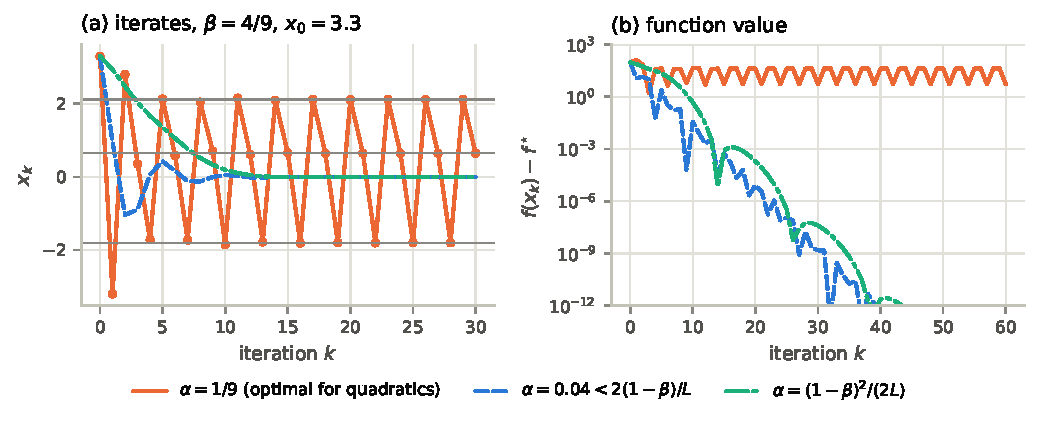
\includegraphics[width=\textwidth]{figures/counterexample.pdf}
\caption{Heavy ball on the strongly convex function of \cref{ex:lrp}, $\beta=\frac49$,
$x_{-1}=x_0=3.3$, exact gradients. (a)~With the quadratic-optimal $\alpha=\frac19$ the iterates
are attracted to the $3$-cycle $\{p_1,p_2,p_3\}$ (grey lines). (b)~The function value then
oscillates forever, while the step sizes allowed by \cref{prop:energy} ($\alpha=0.04$) and by
\cref{thm:master} ($\alpha=(1-\beta)^2/(2L)$) converge.}
\label{fig:lrp}
\end{figure}

\subsection{The map of the parameter plane}\label{sec:map}

\Cref{fig:regions} collects the step-size conditions as regions in the $(\beta,\alpha)$
plane, nested from the most special setting to the most general one:
\begin{itemize}
\item[R4] quadratic $f$, exact gradients: convergence if and only if $\alpha L<2(1+\beta)$
          (\cref{prop:quadratic-stability});
\item[R3] any $L$-smooth $f$, exact gradients: $\alpha L<2(1-\beta)$ suffices
          (\cref{prop:energy});
\item[R2] convex $f$, stochastic gradients: $\alpha L\le\frac{1-\beta}{2}$ suffices
          (\cref{thm:convex});
\item[R1] nonconvex $f$, stochastic gradients: $\alpha L\le\frac{(1-\beta)^2}{2}$ suffices
          (\cref{thm:master,thm:nonconvex}).
\end{itemize}
Panel (b) shows the same regions in terms of the effective step size. There the picture is
strikingly simple: R3 is $\gamma L<2$ and R2 is $\gamma L\le\frac12$, both independent of
$\beta$---momentum with effective step $\gamma$ is as safe as gradient descent with step
$\gamma$---whereas R1 shrinks like $\gamma L\le\frac{1-\beta}{2}$, and R4 (quadratics) grows
without bound as $\beta\to1$. The star (\cref{ex:lrp}) lies in R4 but outside R3, and the
method indeed fails there.

We stress that R1--R3 are \emph{sufficient} conditions. In particular we do not claim that
R1 is necessary for stochastic nonconvex problems; it is the price of a short, general
proof, and in practice larger steps are often used successfully. What the figure does show
is that the question ``does SGDM converge?'' has different answers for different function
classes, and that conclusions drawn from quadratics (R4) do not transfer to general
functions.

\begin{figure}[t]
\centering
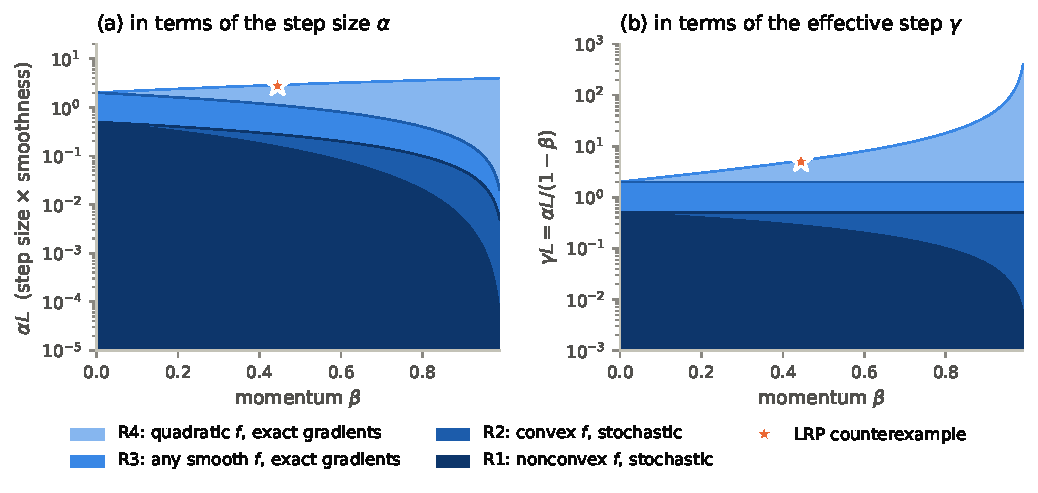
\includegraphics[width=\textwidth]{figures/regions.pdf}
\caption{Where each guarantee holds. Nested regions of admissible parameters,
(a)~in terms of $\alpha L$, (b)~in terms of the effective step $\gamma L=\alpha L/(1-\beta)$
(log scales). R1: \cref{thm:master} (nonconvex, stochastic); R2: \cref{thm:convex}
(convex, stochastic); R3: \cref{prop:energy} (any smooth $f$, exact gradients); R4:
\cref{prop:quadratic-stability} (quadratics, exact gradients). The star marks the
parameters of \cref{ex:lrp}, for which heavy ball cycles on a strongly convex function.}
\label{fig:regions}
\end{figure}

\subsection{Does momentum help?}\label{sec:momentum-help}

The results above give a nuanced answer.
\begin{itemize}
\item \emph{At equal effective step size, SGDM behaves like SGD.} The bounds of
  \cref{sec:convergence} coincide with the SGD bounds up to constants when $\alpha$ is replaced
  by $\gamma$; the noise floor is the same to first order (\cref{prop:noise-floor}); and in
  experiments the trajectories are nearly indistinguishable (\cref{fig:sgd-vs-sgdm}(a)).
  This matches the conclusion of~\cite{liu2020} that SGDM converges as fast as SGD.
\item \emph{At equal raw step size, momentum is a larger step.} It multiplies the effective
  step by $1/(1-\beta)$: faster initial progress, but a floor that is $1/(1-\beta)$ times
  higher (\cref{fig:sgd-vs-sgdm}(b)). Increasing $\beta$ without decreasing $\alpha$ is
  therefore not ``free''.
\item \emph{No worst-case acceleration.} In our analysis the admissible effective step shrinks
  as $\beta\to1$ (R1), and the PL rate $1-\frac{\gamma\mu}{4}$ is no better than that of SGD.
  Acceleration (\cref{sec:circumstances}, ``Momentum on quadratics'') relies on quadratic
  structure and exact gradients; it fails for general strongly convex functions
  (\cref{ex:lrp}) and, for stochastic gradients, there are problems on which the stochastic
  heavy-ball method provably does not improve on SGD~\cite{kidambi2018}.
\end{itemize}
The practical popularity of momentum is therefore better explained by its behaviour on
problems that are locally close to quadratic and ill-conditioned, where the gradient noise
is small relative to the signal, than by worst-case guarantees.

\subsection{When the assumptions fail}

\begin{itemize}
\item \emph{$\beta\ge1$ (no friction).} The roots of $p$ in \cref{prop:quadratic-stability}
  have product $\beta\ge1$, so at least one has modulus $\ge1$: heavy ball does not converge
  even on $\frac12x^2$. The extrapolated point and the effective step size are undefined.
  The condition $\beta<1$ is necessary.
\item \emph{Noise growing with the gradient},
  $\Ek\norm{g_k-\nabla f(x_k)}^2\le\sigma^2+M\norm{\nabla f(x_k)}^2$: all results remain
  valid with the step-size condition tightened by the factor $1+M$
  (\cref{rem:extensions}(ii)).
\item \emph{Infinite variance (heavy-tailed noise).} \Cref{as:variance} fails and the bounds
  above are vacuous; techniques such as gradient clipping are then used. This is beyond the
  scope of this report.
\item \emph{Biased gradients.} Unbiasedness (\cref{as:unbiased}) is used in
  \cref{lem:z-descent,lem:velocity}. With a bias, both lemmas acquire additional error
  terms and convergence can only be guaranteed up to a neighbourhood whose size depends on
  the bias.
\item \emph{Non-smooth $f$.} Without \cref{as:smooth} there is no descent lemma; momentum
  methods for non-smooth (weakly convex) problems require different tools,
  see~\cite{mai2020}.
\end{itemize}

\subsection{Summary: a checklist}

SGDM achieves the SGD-style expected decrease, and hence the convergence guarantees of
\cref{sec:convergence}, under the following circumstances.
\begin{enumerate}
\item \textbf{The problem:} $f$ is $L$-smooth and bounded below; the stochastic gradients are
  unbiased with bounded variance $\sigma^2$ (\cref{as:smooth,as:lower,as:unbiased,as:variance}).
\item \textbf{The momentum:} $\beta\in[0,1)$---friction must be present.
\item \textbf{The step size, measured as the effective step $\gamma=\alpha/(1-\beta)$:}
  \begin{itemize}
  \item general nonconvex, stochastic: $\gamma\le\frac{1-\beta}{2L}$, i.e.\ $\alpha\le\frac{(1-\beta)^2}{2L}$;
  \item convex, stochastic: $\gamma\le\frac{1}{2L}$;
  \item any smooth $f$, exact gradients: $\gamma<\frac2L$.
  \end{itemize}
\item \textbf{The target:} with a constant step one reaches a noise region of size
  $O(\gamma\sigma^2)$, which is unavoidable (\cref{prop:noise-floor}); to reach accuracy
  $\eps^2$ in $\min_k\E\norm{\nabla f(x_k)}^2$ choose $\gamma\propto1/\sqrt K$
  (\cref{cor:rate}), or use decaying steps (\cref{thm:diminishing}) for asymptotic convergence.
\item \textbf{Linear rates} need additional structure such as the PL inequality or strong
  convexity (\cref{thm:pl}); the rate is $1-\gamma\mu/4$.
\item \textbf{Beware of quadratic intuition:} parameters that are stable or even optimal for
  quadratics can make the method cycle on a strongly convex function (\cref{ex:lrp}).
\end{enumerate}

% ======================================================================
\section{Numerical illustrations}\label{sec:experiments}
% ======================================================================

The experiments below illustrate the theorems; they are not needed for the proofs. All of
them run Algorithm~1 in heavy-ball form (the implementation in
\texttt{experiments/common.py} is a direct transcription of the update
$v_{k+1}=\beta v_k-\alpha_kg_k$, $x_{k+1}=x_k+v_{k+1}$), vectorized over independent runs;
expectations are estimated by averaging over runs. Every figure is produced by one script
(\cref{app:reproduce}).

\paragraph{Test problems.}
\begin{enumerate}[label=(P\arabic*)]
\item \emph{Quadratic:} $f(x)=\frac h2x^2$ with $h=L=1$; stochastic gradient
  $g=hx+\xi$, $\xi\sim\mathcal N(0,\sigma^2)$.
\item \emph{Nonconvex PL function:} $f(x)=\sum_{i=1}^{10}(x_i^2+3\sin^2x_i)$ on $\R^{10}$
  ($L=8$, $\mu=\frac1{32}$, $\fs=0$, \cref{lem:pl-facts}(c)); stochastic gradient
  $g=\nabla f(x)+\xi$ with $\xi\sim\mathcal N(0,\frac{\sigma^2}{10}I)$, so that
  $\E\norm{\xi}^2=\sigma^2$.
\item \emph{Nonconvex logistic regression:}
  $f(x)=\frac1n\sum_{i=1}^n\log\bigl(1+e^{-b_ia_i^\top x}\bigr)+\lambda\sum_{j=1}^d\frac{x_j^2}{1+x_j^2}$
  with $n=1000$, $d=20$, $\lambda=0.1$, features $a_i\sim\mathcal N(0,I_d)$, and labels
  $b_i\in\{\pm1\}$ drawn from the logistic model with a random parameter vector. The
  regularizer is nonconvex. Stochastic gradients use one uniformly sampled example (mini-batch
  size $1$); they are unbiased with bounded variance, and $f$ is $L$-smooth with
  $L\le\frac{\norm{A}_2^2}{4n}+2\lambda\approx0.515$, where $A$ has rows $a_i^\top$. All runs start
  at $x_0=(-1,\dots,-1)$.
\item \emph{The function of \cref{ex:lrp}} (strongly convex, exact gradients).
\end{enumerate}

\paragraph{Potential versus function value (\cref{fig:potential}).} On (P1) with $\beta=0.9$
and the largest step allowed by \cref{thm:master}, $\alpha=(1-\beta)^2/(2L)=0.005$, the
function value $f(x_k)$ is not monotone even without noise, because the iterate overshoots
(panel (b)); the potential $\Phi_k$ decreases at every step, as guaranteed by
\cref{cor:when-decrease}. (The script also checks this monotonicity numerically.) With noise
(panel (c)), the empirical floor of $\E f(x_k)$ is $0.01252$, matching the exact value of
\cref{prop:noise-floor} to four digits.

\begin{figure}[t]
\centering
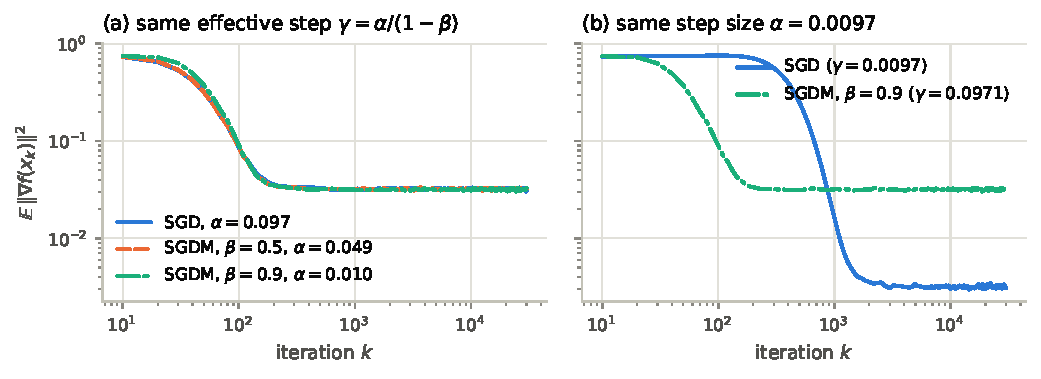
\includegraphics[width=\textwidth]{figures/sgd_vs_sgdm.pdf}
\caption{SGD versus SGDM on the nonconvex logistic regression problem (P3), mean of
$\norm{\nabla f(x_k)}^2$ over $100$ runs (lightly smoothed). (a)~Same effective step
$\gamma=\frac{1-0.9}{2L}$, inside the range of \cref{thm:master} for every $\beta$ shown: the
three methods are indistinguishable. (b)~Same raw step $\alpha=\frac{(1-0.9)^2}{2L}$:
momentum $\beta=0.9$ makes the effective step $10$ times larger, so it converges faster at
first but stalls at a $10$ times higher noise floor.}
\label{fig:sgd-vs-sgdm}
\end{figure}

\paragraph{SGD versus SGDM (\cref{fig:sgd-vs-sgdm}).} On (P3), SGD and SGDM with
$\beta\in\{0.5,0.9\}$ run at the same effective step size produce practically identical
curves (panel (a)), including the level of the noise floor: SGDM behaves like SGD with step
$\gamma$, as the parallel between \cref{lem:sgd-step} and \cref{thm:master} suggests. At
the same raw step size (panel (b)), momentum is simply a ten times larger step: faster
initial progress, ten times higher floor, consistent with \cref{prop:noise-floor}.

\begin{figure}[t]
\centering
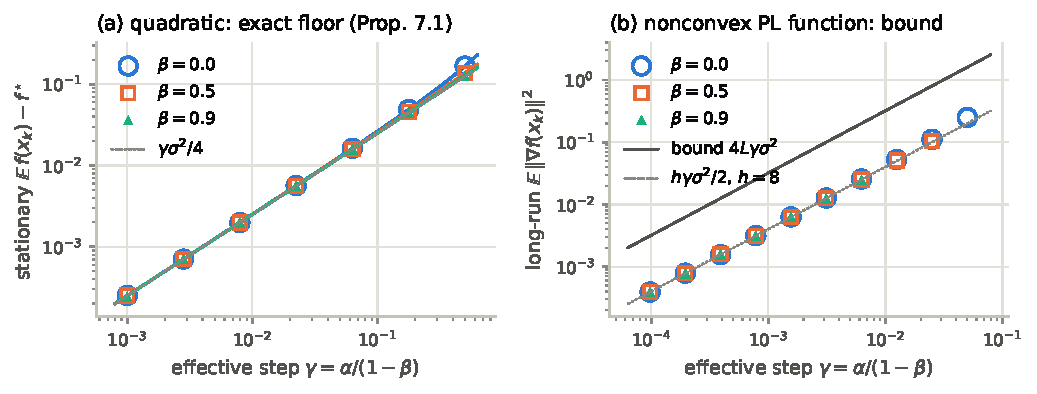
\includegraphics[width=\textwidth]{figures/noise_floor.pdf}
\caption{The noise floor with a constant step scales like $\gamma\sigma^2$ and, to first
order, depends on $(\alpha,\beta)$ only through $\gamma$ (markers for different $\beta$ lie
on top of each other). (a)~Quadratic (P1), $\sigma=1$: empirical stationary $\E f(x_k)$
(markers; $4000$ runs) and the exact formula \eqref{eq:noise-floor} (lines). (b)~Nonconvex
PL function (P2), $\sigma=1$: long-run $\E\norm{\nabla f(x_k)}^2$ ($400$ runs) for step
sizes inside the range of \cref{thm:master}, the bound $4L\gamma\sigma^2$ of
\cref{thm:nonconvex} (as $K\to\infty$), and the local quadratic prediction
$h\gamma\sigma^2/2$ with $h=f''(0)=8$.}
\label{fig:noise-floor}
\end{figure}

\paragraph{The noise floor (\cref{fig:noise-floor}).} For each $\beta\in\{0,0.5,0.9\}$ and a
range of effective step sizes we run the method from the minimizer until it reaches
stationarity and average the quantity of interest over time and runs. On the quadratic,
the measurements agree with \eqref{eq:noise-floor} to within $2\%$ for every $(\gamma,\beta)$.
On the nonconvex PL function, the measured floors lie on the line $h\gamma\sigma^2/2$
predicted by the local quadratic approximation at the minimizer, and about a factor $8$
below the bound $4L\gamma\sigma^2$ of \cref{thm:nonconvex}: the theorem has the correct
dependence on $\gamma$ and $\sigma$, with a pessimistic constant. In both panels the points for
different $\beta$ coincide.

\begin{figure}[t]
\centering
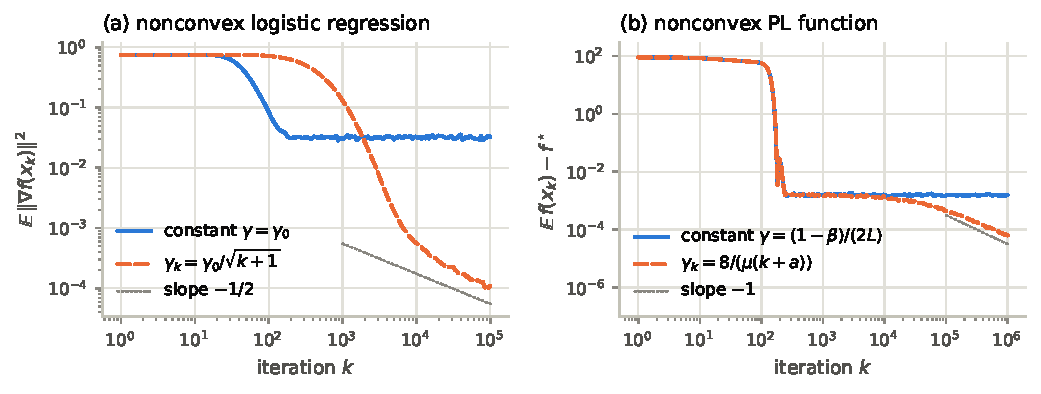
\includegraphics[width=\textwidth]{figures/diminishing.pdf}
\caption{Diminishing step sizes remove the noise floor ($\beta=0.9$; both schedules start
from the same $\gamma_0=\frac{1-\beta}{2L}$). (a)~Nonconvex logistic regression (P3), $50$ runs:
constant step versus $\gamma_k=\gamma_0/\sqrt{k+1}$ (\cref{thm:diminishing}(c)). (b)~Nonconvex
PL function (P2), $100$ runs: constant step versus $\gamma_k=\frac8{\mu(k+a)}$ with
$a=\frac{16L}{\mu(1-\beta)}$ (\cref{cor:pl-decay}); the dotted lines have slopes $-\frac12$ and
$-1$.}
\label{fig:diminishing}
\end{figure}

\paragraph{Diminishing steps (\cref{fig:diminishing}).} With a constant step the error
stalls at its noise floor; with the schedules of \cref{thm:diminishing,cor:pl-decay} it keeps
decreasing. On the logistic problem the gradient norm decreases roughly like $k^{-1/2}$,
which is the order of $\gamma_k$; on the PL function the optimality gap eventually decreases
like $1/k$, as predicted by \cref{cor:pl-decay}. (The theoretical schedule for the PL function
starts slowly because the certified PL constant $\mu=\frac1{32}$ is much smaller than the
local curvature at the minimizer.) Note also the non-monotone transient around $k\approx200$
in panel (b), another manifestation of overshooting.

\paragraph{The counterexample (\cref{fig:lrp}).} On the function of \cref{ex:lrp},
quadratic-optimal parameters lead to the predicted $3$-cycle, while the step sizes allowed by
\cref{prop:energy} and \cref{thm:master} converge. The script verifies the cycle in exact
rational arithmetic.

% ======================================================================
\section{Conclusion}\label{sec:conclusion}
% ======================================================================

The standard analysis of SGD rests on a one-step expected decrease of the function value.
For SGD with momentum the function value is the wrong yardstick, because momentum makes
the iterates overshoot. The report's main message fits in three sentences.

\begin{enumerate}
\item \emph{SGDM is SGD on the extrapolated points.} The points
  $z_k=x_k+\frac{\beta}{1-\beta}(x_k-x_{k-1})$, where the ball would come to rest if the
  force were switched off, follow exact SGD steps $z_{k+1}=z_k-\gamma g_k$ with the effective
  step size $\gamma=\alpha/(1-\beta)$; only the gradient is evaluated at the nearby point $x_k$
  (\cref{lem:z}).
\item \emph{A potential decreases in expectation, exactly as $f$ does for SGD.} The
  potential $\Phi_k=f(z_k)-\fs+\frac{L\beta^2}{2(1-\beta)^2}\norm{x_k-x_{k-1}}^2$ satisfies
  $\Ek\Phi_{k+1}\le\Phi_k-\frac\gamma4\norm{\nabla f(x_k)}^2+L\gamma^2\sigma^2$ whenever
  $\alpha\le(1-\beta)^2/(2L)$: friction must dissipate kinetic energy faster than the gradient
  mismatch creates error (\cref{thm:master}).
\item \emph{Everything else follows as for SGD.} Telescoping gives the $O(1/\sqrt K)$
  nonconvex rate, diminishing steps give asymptotic convergence, the PL inequality gives
  linear convergence to a noise floor, and convexity relaxes the step-size condition to
  $\gamma\le1/(2L)$ (\cref{sec:convergence}).
\end{enumerate}

As for \emph{when} convergence holds (\cref{sec:circumstances}): the momentum must satisfy
$\beta<1$; the step size must be small in terms of the effective step $\gamma$, with a
threshold that depends on the function class (\cref{fig:regions}); a constant step only
reaches a noise floor of order $\gamma\sigma^2$, which is unavoidable and the same as for SGD
(\cref{prop:noise-floor}); and stability or optimality on quadratics does not imply
convergence on general functions (\cref{ex:lrp}). In the worst case, momentum neither
accelerates nor slows down SGD once the step sizes are compared on the right scale.


\appendix
% ======================================================================
\section{Linear recurrences and powers of \texorpdfstring{$2\times2$}{2x2} matrices}\label{app:linear}
% ======================================================================

These two standard facts are used in \cref{prop:noise-floor,prop:quadratic-stability}.

\begin{lemma}[Second-order linear recurrences]\label{lem:recurrence}
Let $a\in\R$, $b\ne0$, and let $\lambda_1,\lambda_2\in\mathbb C$ be the roots of
$p(\lambda)=\lambda^2-a\lambda+b$. The solutions $(x_k)_{k\ge-1}$ of
$x_{k+1}=ax_k-bx_{k-1}$ ($k\ge0$) are exactly the sequences
\begin{enumerate}[label=\textup{(\roman*)}]
\item $x_k=c_1\lambda_1^k+c_2\lambda_2^k$ with $c_1,c_2\in\mathbb C$, if $\lambda_1\ne\lambda_2$;
\item $x_k=(c_1+c_2k)\lambda_1^k$ with $c_1,c_2\in\mathbb C$, if $\lambda_1=\lambda_2$.
\end{enumerate}
\end{lemma}

\begin{proof}
\emph{These are solutions.} For a root $\lambda$,
$\lambda^{k+1}-a\lambda^k+b\lambda^{k-1}=\lambda^{k-1}p(\lambda)=0$, and sums of solutions
are solutions. In case (ii), $\lambda_1=a/2$ and $b=\lambda_1^2$ (product of the roots), and
\[
  (k+1)\lambda_1^{k+1}-ak\lambda_1^k+b(k-1)\lambda_1^{k-1}
  =\lambda_1^{k-1}\bigl[k\,p(\lambda_1)+\lambda_1^2-b\bigr]=0 .
\]
\emph{There are no others.} A solution is determined by $(x_{-1},x_0)$, so it suffices to
show that every pair $(x_{-1},x_0)$ is attained. In case (i) we need
$c_1\lambda_1^{-1}+c_2\lambda_2^{-1}=x_{-1}$, $c_1+c_2=x_0$; the determinant of this linear
system is $\lambda_2^{-1}-\lambda_1^{-1}=\frac{\lambda_1-\lambda_2}{\lambda_1\lambda_2}\ne0$
(the roots are nonzero because $\lambda_1\lambda_2=b\ne0$). In case (ii) we need
$(c_1-c_2)\lambda_1^{-1}=x_{-1}$ and $c_1=x_0$, which has the solution $c_1=x_0$,
$c_2=x_0-\lambda_1x_{-1}$.
\end{proof}

When $b=\beta=0$ the heavy-ball recurrence reduces to $x_{k+1}=ax_k$, with solutions
$x_k=a^kx_0$; the arguments of \cref{prop:quadratic-stability} apply verbatim with the roots
$a$ and $0$.

\begin{lemma}[Powers of a $2\times2$ matrix]\label{lem:matrix-powers}
Let $M$ be a real $2\times2$ matrix whose eigenvalues satisfy
$\max\{|\lambda_1|,|\lambda_2|\}<\rho<1$. Then there is a constant $C_M$ such that every entry
of $M^k$ is at most $C_M\rho^k$ in absolute value, for all $k\ge0$. Consequently, for any
$2\times2$ matrices $C_0,Q$, we have $M^kC_0(M^\top)^k\to0$, and the series
$\sum_{j\ge0}M^jQ(M^\top)^j$ converges.
\end{lemma}

\begin{proof}
If $\lambda_1\ne\lambda_2$, $M$ is diagonalizable over $\mathbb C$: $M=V\,\mathrm{diag}(\lambda_1,\lambda_2)V^{-1}$,
so $M^k=V\,\mathrm{diag}(\lambda_1^k,\lambda_2^k)V^{-1}$ and its entries are bounded by a constant
times $\max_i|\lambda_i|^k\le\rho^k$. If $\lambda_1=\lambda_2=\lambda$, then either
$M=\lambda I$, or $M=VJV^{-1}$ with the Jordan block $J=\begin{pmatrix}\lambda&1\\0&\lambda\end{pmatrix}$,
for which $J^k=\begin{pmatrix}\lambda^k&k\lambda^{k-1}\\0&\lambda^k\end{pmatrix}$; since
$k|\lambda|^{k-1}/\rho^k\to0$, the entries of $M^k$ are again bounded by a constant times
$\rho^k$. The entries of $M^jQ(M^\top)^j$ are then bounded by a constant times $\rho^{2j}$, so
the series converges absolutely, and similarly $M^kC_0(M^\top)^k\to0$.
\end{proof}

% ======================================================================
\section{Reproducing the figures}\label{app:reproduce}
% ======================================================================

The repository contains the \LaTeX{} source of this report (\texttt{report/}) and the
Python code for all figures (\texttt{experiments/}, requiring \texttt{numpy} and
\texttt{matplotlib}). From the repository root:
\begin{verbatim}
  pip install -r experiments/requirements.txt
  python experiments/run_all.py          # regenerates report/figures/*.pdf
  cd report && latexmk -pdf main.tex     # rebuilds the PDF
\end{verbatim}
or simply \texttt{make}. The scripts and the figures they produce are:
\begin{center}\small
\begin{tabular}{@{}lll@{}}
\toprule
script & figure & content\\
\midrule
\texttt{potential.py} & \cref{fig:potential} & $f(x_k)$ versus $\Phi_k$; checks monotonicity of $\Phi_k$\\
\texttt{regions.py} & \cref{fig:regions} & parameter regions\\
\texttt{sgd\_vs\_sgdm.py} & \cref{fig:sgd-vs-sgdm} & SGD versus SGDM on (P3)\\
\texttt{noise\_floor.py} & \cref{fig:noise-floor} & noise floor versus $\gamma$\\
\texttt{diminishing.py} & \cref{fig:diminishing} & diminishing step sizes\\
\texttt{counterexample.py} & \cref{fig:lrp} & the $3$-cycle of \cref{ex:lrp}, verified exactly\\
\bottomrule
\end{tabular}
\end{center}
All random seeds are fixed, so the figures are reproducible.


\begin{thebibliography}{99}
\small

\bibitem{bertsekas2000}
D.~P. Bertsekas and J.~N. Tsitsiklis.
\newblock Gradient convergence in gradient methods with errors.
\newblock \emph{SIAM Journal on Optimization}, 10(3):627--642, 2000.

\bibitem{bottou2018}
L.~Bottou, F.~E. Curtis, and J.~Nocedal.
\newblock Optimization methods for large-scale machine learning.
\newblock \emph{SIAM Review}, 60(2):223--311, 2018.

\bibitem{gadat2018}
S.~Gadat, F.~Panloup, and S.~Saadane.
\newblock Stochastic heavy ball.
\newblock \emph{Electronic Journal of Statistics}, 12(1):461--529, 2018.

\bibitem{ghadimi2015}
E.~Ghadimi, H.~R. Feyzmahdavian, and M.~Johansson.
\newblock Global convergence of the heavy-ball method for convex optimization.
\newblock In \emph{Proceedings of the European Control Conference (ECC)}, 2015.

\bibitem{ghadimilan2013}
S.~Ghadimi and G.~Lan.
\newblock Stochastic first- and zeroth-order methods for nonconvex stochastic programming.
\newblock \emph{SIAM Journal on Optimization}, 23(4):2341--2368, 2013.

\bibitem{karimi2016}
H.~Karimi, J.~Nutini, and M.~Schmidt.
\newblock Linear convergence of gradient and proximal-gradient methods under the
  {P}olyak--{\L}ojasiewicz condition.
\newblock In \emph{Machine Learning and Knowledge Discovery in Databases (ECML PKDD)}, 2016.

\bibitem{kidambi2018}
R.~Kidambi, P.~Netrapalli, P.~Jain, and S.~M. Kakade.
\newblock On the insufficiency of existing momentum schemes for stochastic optimization.
\newblock In \emph{International Conference on Learning Representations (ICLR)}, 2018.

\bibitem{lessard2016}
L.~Lessard, B.~Recht, and A.~Packard.
\newblock Analysis and design of optimization algorithms via integral quadratic constraints.
\newblock \emph{SIAM Journal on Optimization}, 26(1):57--95, 2016.

\bibitem{liu2020}
Y.~Liu, Y.~Gao, and W.~Yin.
\newblock An improved analysis of stochastic gradient descent with momentum.
\newblock In \emph{Advances in Neural Information Processing Systems (NeurIPS)}, 2020.

\bibitem{mai2020}
V.~V. Mai and M.~Johansson.
\newblock Convergence of a stochastic gradient method with momentum for non-smooth
  non-convex optimization.
\newblock In \emph{International Conference on Machine Learning (ICML)}, 2020.

\bibitem{polyak1964}
B.~T. Polyak.
\newblock Some methods of speeding up the convergence of iteration methods.
\newblock \emph{USSR Computational Mathematics and Mathematical Physics}, 4(5):1--17, 1964.

\bibitem{robbins1951}
H.~Robbins and S.~Monro.
\newblock A stochastic approximation method.
\newblock \emph{The Annals of Mathematical Statistics}, 22(3):400--407, 1951.

\bibitem{robbinssiegmund1971}
H.~Robbins and D.~Siegmund.
\newblock A convergence theorem for non negative almost supermartingales and some applications.
\newblock In \emph{Optimizing Methods in Statistics}, pages 233--257. Academic Press, 1971.

\bibitem{sebbouh2021}
O.~Sebbouh, R.~M. Gower, and A.~Defazio.
\newblock Almost sure convergence rates for stochastic gradient descent and stochastic heavy ball.
\newblock In \emph{Conference on Learning Theory (COLT)}, 2021.

\bibitem{sutskever2013}
I.~Sutskever, J.~Martens, G.~Dahl, and G.~Hinton.
\newblock On the importance of initialization and momentum in deep learning.
\newblock In \emph{International Conference on Machine Learning (ICML)}, 2013.

\bibitem{yang2016}
T.~Yang, Q.~Lin, and Z.~Li.
\newblock Unified convergence analysis of stochastic momentum methods for convex and
  non-convex optimization.
\newblock arXiv:1604.03257, 2016.

\bibitem{yu2019}
H.~Yu, R.~Jin, and S.~Yang.
\newblock On the linear speedup analysis of communication efficient momentum {SGD} for
  distributed non-convex optimization.
\newblock In \emph{International Conference on Machine Learning (ICML)}, 2019.

\bibitem{zavriev1993}
S.~K. Zavriev and F.~V. Kostyuk.
\newblock Heavy-ball method in nonconvex optimization problems.
\newblock \emph{Computational Mathematics and Modeling}, 4:336--341, 1993.

\end{thebibliography}


\end{document}
